\documentclass[12pt]{aghdpl}

\newtheorem{theorem}{Twierdzenie}
\newtheorem{definition}{Definicja}
\newtheorem{lemma}{Lemat}
\newtheorem{corollary}{Wniosek}

\usepackage{diagbox}
\usepackage{pgfplots}
\pgfplotsset{compat=1.18}

\usepackage{minted}

%---------------------------------------------------------------------------

\author{Piotr Karaś}
\shortauthor{P. Karaś}

%\titlePL{Przygotowanie bardzo długiej i pasjonującej pracy dyplomowej w~systemie~\LaTeX}
%\titleEN{Preparation of a very long and fascinating bachelor or master thesis in \LaTeX}

\titlePL{Ewaluacja metod odkrywania gramatyki języka formalnego}
\titleEN{Evaluation of Grammar Induction Methods}

\shorttitlePL{Ewaluacja metod odkrywania gramatyki języka formalnego}
\shorttitleEN{Evaluation of Grammar Induction Methods}

% Dopuszczalne wartości[1,2]:
% * "Projekt dyplomowy" - na koniec studiów I stopnia
% * "Praca dyplomowa" - na koniec studiów II stopnia
% [1] Zasady dyplomowania w roku akademickim 2020/2021 (Decyzja Dziekana WEAIiIB nr 16/2020 z dnia 9 grudnia 2020 roku)
% [2] Załącznik nr 1a) do Decyzji nr 16/2020 Dziekana Wydziału EAIiIB z dnia 09 grudnia 2020 r.
\thesistype{Praca Inżynierska}

\supervisor{dr inż. Mateusz Ślażyński}

\degreeprogramme{Informatyka i Systemy Inteligentne}

\date{2024}

%\department{Katedra Informatyki Stosowanej}
%\department{Department of Applied Computer Science}

\faculty{Wydział Elektrotechniki, Automatyki, Informatyki i Inżynierii Biomedycznej}
%\faculty{Faculty of Electrical Engineering, Automatics, Computer Science and Biomedical Engineering}

\acknowledgements{Składam serdeczne podziękowania dr inż. Mateuszowi Ślażyńskiemu za opiekę \break naukową podczas realizacji pracy.}


\begin{document}
    \titlepages
    \RedefinePlainStyle
    
    \setcounter{tocdepth}{2}
    \tableofcontents
    \clearpage
    
    \chapter{Wprowadzenie}  
\label{cha:wprowadzenie}  

Każdy internauta musiał kiedyś nauczyć się, jak wygląda poprawny adres e-mail. Początkowo użytkownik wpisywał różne frazy w formularzu rejestracyjnym, dowiadując się, czy dana sekwencja znaków jest akceptowana przez system. Przykładowo, mógł sprawdzić, że \texttt{jan.kowalski@example.com} zostaje zaakceptowany, podczas gdy \texttt{jan.kowalski@com} lub \texttt{jan.kowalski.example.com} są odrzucane. Mógł również znać kilka adresów, przykładowo swoich przyjaciół. Na podstawie odrzuconych formularzy oraz znanych już adresów e-mail użytkownik wykształcał pewną intuicję dotyczącą reguł rządzących poprawnymi adresami e-mail. Ten proces nauki jest przykładem indukcji gramatyki regularnej. 

Uczenie indukcyjne (\textit{inductive learning}) jest jednym z podstawowych podejść w dziedzinie uczenia maszynowego, którego celem jest odnalezienie ogólnych reguł na podstawie zbioru przykładów. Proces ten polega na analizie dostępnych danych wejściowych w celu wykrycia ukrytych wzorców i struktur, które mogą zostać uogólnione do postaci formalnego modelu. Modele takie znajdują zastosowanie w szerokim zakresie problemów, od klasyfikacji i przewidywania po modelowanie języków formalnych i systemów dynamicznych.  

Jednym z obszarów zastosowania uczenia indukcyjnego jest indukcja gramatyk formalnych, która stanowi istotne zagadnienie zarówno w uczeniu maszynowym, jak i teorii automatów. Jej celem jest odtworzenie reguł opisujących język formalny na podstawie skończonego zbioru danych wejściowych. Proces ten pozwala na budowę modeli, takich jak automaty skończone lub gramatyki formalne, które mogą zostać zastosowane do analizy danych sekwencyjnych, rozpoznawania wzorców, przetwarzania języka naturalnego oraz weryfikacji systemów.  

Podstawą teoretyczną badań nad indukcją gramatyk jest koncepcja identyfikacji w granicy (\textit{identification in the limit}) \cite{GOLD1967447}. Określa ona warunki, w których algorytm jest zdolny do poprawnej rekonstrukcji struktury języka na podstawie skończonej liczby przykładów. Chociaż wyniki teoretyczne dostarczają istotnych gwarancji dotyczących poprawności algorytmów, praktyczne aspekty indukcji gramatyk pozostają przedmiotem dalszych badań, zwłaszcza w kontekście danych rzeczywistych, które często są obarczone szumem lub są niepełne.

%---------------------------------------------------------------------------

\section{Cele pracy}
\label{sec:celePracy}

% Szczegółowe określenie celów badania lub projektowania.
% Zakres pracy, czyli określenie granic projektu (co zostanie wykonane, a co nie).
% Problemy, które praca ma rozwiązać.  

Celem niniejszej pracy jest ewaluacja i porównanie wybranych algorytmów indukcji gramatyk formalnych. Przeanalizowane zostaną zarówno algorytmy klasyczne, takie jak \textit{L*} i \textit{RPNI}, jak i bardziej zaawansowane podejścia, w tym probabilistyczny algorytm \textit{ALERGIA} oraz metoda oparta na algorytmach genetycznych (\textit{GIG}). Badania koncentrują się na dokładności generowanych modeli, ich efektywności obliczeniowej oraz zdolności do uogólniania informacji przy niepełnych lub zaszumionych danych.

Przedstawione badania mają na celu nie tylko porównanie istniejących algorytmów, ale również dostarczenie praktycznych wskazówek dotyczących ich zastosowania w zależności od charakterystyki danych i wymagań aplikacyjnych. Praca stanowi krok w kierunku lepszego zrozumienia możliwości oraz ograniczeń metod indukcji gramatyk, otwierając jednocześnie perspektywy dla dalszych badań w tym obszarze.  

W ramach pracy zbudowane zostanie środowisko do ewaluacji metod indukcji gramatyk, umożliwiające porównanie różnych technik pod kątem ich wydajności i zastosowań praktycznych. Eksperymenty obejmują analizę danych syntetycznych, a wyniki zostaną ocenione pod względem jakości generowanych modeli, złożoności czasowej oraz pamięciowej. 

%---------------------------------------------------------------------------

\section{Zawartość pracy}
\label{sec:zawartoscPracy}

% Przegląd literatury (teoretyczne podstawy pracy)
% Omówienie istniejących prac i badań związanych z tematem.
% Podstawy teoretyczne, które są niezbędne do zrozumienia tematu.
% Analiza istniejących rozwiązań, narzędzi lub metod stosowanych w dziedzinie.
% Krótki przegląd struktury pracy.

Niniejsza praca jest poświęcona analizie oraz porównaniu algorytmów indukcji gramatyk regularnych. Jej celem jest przedstawienie teoretycznych podstaw, metodologii oraz wyników eksperymentalnych dotyczących wybranych algorytmów. Praca składa się z sześciu rozdziałów, które szczegółowo opisano poniżej.

Pierwszy rozdział stanowi wprowadzenie do tematyki pracy. Przedstawiono w nim ogólne informacje dotyczące problematyki indukcji gramatyk formalnych. Omówiono cele pracy oraz zarysowano jej strukturę, wskazując na kluczowe aspekty analizowanych algorytmów. 

Drugi rozdział opisuje metodykę badań, w tym kryteria wyboru algorytmów oraz przyjęte założenia eksperymentalne. Zawiera również szczegółowy opis sposobu oceny skuteczności analizowanych metod oraz charakterystykę danych użytych w eksperymentach. 

Trzeci rozdział jest najobszerniejszą częścią pracy i zawiera szczegółowe opisy wybranych algorytmów. Przedstawiono w nim cztery kluczowe metody: \textit{L*}, \textit{RPNI}, \textit{GIG} oraz \textit{ALERGIA}. Każdy z tych algorytmów został opisany pod kątem swojej metody działania, formalizacji, złożoności obliczeniowej oraz zilustrowany praktycznymi przykładami zastosowań. Omówiono również różnice pomiędzy podejściem genetycznym a zachłannym, które są kluczowe w kontekście algorytmu \textit{GIG}. Dodatkowo przedstawiono krótki przegląd pozostałych algorytmów, które nie zostały uwzględnione w szczegółowej analizie.

Czwarty rozdział skupia się na eksperymentach przeprowadzonych w celu oceny skuteczności opisanych algorytmów. Opisano specyfikę eksperymentów, zestawy danych oraz metryki służące do oceny wyników.

W piątym rozdziale omówiono wyniki eksperymentów. Przeprowadzono analizę uzyskanych rezultatów, porównując algorytmy pod kątem ich zdolności do generalizacji, jakości wyników oraz efektywności obliczeniowej. Przedstawiono również ograniczenia poszczególnych metod oraz wskazano potencjalne kierunki ich ulepszenia.

Ostatni, szósty rozdział, zawiera podsumowanie pracy oraz wnioski płynące z przeprowadzonych badań. Zawarto w nim także możliwości wykorzystania badanych algorytmów w praktycznych zastosowaniach.

Przegląd literatury, podstawy teoretyczne oraz analiza istniejących rozwiązań zostały zintegrowane z poszczególnymi rozdziałami, co zapewnia spójność tematyczną i logiczną narrację całej pracy.

    \chapter{Algorytmy}
\label{cha:algorytmy}

Istnieje wiele algorytmów do odkrywania struktury języka formalnego. Na przestrzeni lat powstało również wiele podejść i metod, które pomagają tworzyć zarówno rozwiązania ogólne, jak i te szczególnie efektywne w swojej niszy. Z uwagi na dużą liczbę dostępnych algorytmów zdecydowano się na ich ograniczony podzbiór, który wykorzystano w pracy. Są to \textit{L*}, \textit{RPNI}, \textit{GIG} i \textit{ALERGIA}, opisane kolejno w sekcjach \ref{sec:l-star}, \ref{sec:rpni}, \ref{sec:gig} i \ref{sec:alergia}. To właśnie te algorytmy przedstawiono jako pierwsze. Następnie krótko omówiono pozostałe algorytmy, które zostały uznane za interesujące, oraz wyjaśniono, dlaczego nie zdecydowano się na ich użycie.

\newenvironment{observationtable}[1][Tabela Obserwacji]{
  \begin{center}
  \renewcommand{\arraystretch}{1.3}
  \textbf{#1}\vspace{0.5em} \\
  \begin{tabular}{|c|c|c|}
  \hline
}{
  \hline
  \end{tabular}
  \end{center}
}

\section{Algorytm \textit{L*}}
\label{sec:l-star}

Algorytm \textit{L*} \cite{L_STAR} wyróżnia się na tle innych algorytmów do odkrywania gramatyki języka regularnego użytych w pracy dzięki swojemu podejściu do uczenia. Większość innych algorytmów opiera się wyłącznie na przykładach pozytywnych lub zarówno na przykładach pozytywnych, jak i negatywnych. Algorytm \textit{L*} wyłamuje się z tej konwencji, wykorzystując zapytania oraz kontrprzykłady do procesu nauki.

Model algorytmu składa się z dwóch aktorów: \textbf{nauczyciela} oraz \textbf{ucznia}. Jego celem jest skonstruowanie minimalnego deterministycznego automatu skończonego (DFA), który rozpoznaje dany język regularny na podstawie ograniczonych interakcji między dwoma uczestnikami procesu.

\subsection{Metoda}

Konstruowanie minimalnego automatu deterministycznego (DFA), który akceptuje język \( L \), odbywa się przy pomocy dwóch rodzajów zapytań:
\begin{enumerate}
    \item \textbf{Zapytania o członkostwo (Membership Queries, \textit{MQ}):} Uczeń pyta, czy słowo \( w \) należy do języka \( L \). Nauczyciel odpowiada „tak” (\( w \in L \)) lub „nie” (\( w \notin L \)).
    \item \textbf{Zapytania o równoważność (Equivalence Queries, \textit{EQ}):} Uczeń przedstawia hipotezę \( H \), reprezentującą język \( L(H) \), i pyta, czy \( L(H) = L \). Jeśli hipoteza jest niepoprawna, nauczyciel dostarcza kontrprzykład \( w \), dla którego \( w \in L \) i \( w \notin L(H) \), lub \( w \notin L \) i \( w \in L(H) \).
\end{enumerate}

Dla poprawnego działania algorytmu wymagane jest, aby nauczyciel mógł udzielać prawdziwych odpowiedzi na oba rodzaje zadawanych pytań. Nauczyciela często nazywa się również \textbf{wyrocznią}, co jest skrótem myślowym, ponieważ formalnie nauczyciel składa się z pary \textbf{wyroczni (oracles)}: \textit{MQ} i \textit{EQ}. Zazwyczaj to na użytkowniku algorytmu spoczywa odpowiedzialność za określenie nauczyciela, co wymaga już na wstępie posiadania pewnej wiedzy na temat danego języka. Jest to największe ograniczenie w zastosowaniu algorytmu \textit{L*}.

Proces algorytmu \textit{L*} opiera się na iteracyjnym konstruowaniu \textbf{tabeli obserwacji (Observation Table)}, która gromadzi informacje o języku L uzyskane na podstawie zapytań typu \textit{MQ}. Na podstawie zawartości tabeli formułowane są kolejne hipotezy dotyczące automatu DFA, które następnie poddawane są weryfikacji za pomocą zapytań typu \textit{EQ}.

Główne kroki algorytmu:
\begin{enumerate}
    \item \textbf{Inicjalizacja:} Algorytm rozpoczyna od utworzenia tabeli obserwacji wykorzystując minimalne zbiory prefiksów (\( S \)) i sufiksów (\( E \)).
    \item \textbf{Sprawdzanie domknięcia i spójności:} Algorytm weryfikuje, czy tabela obserwacji spełnia wymagania:
    \begin{itemize}
        \item \textbf{Domknięcie:} Każdy prefiks prowadzi do jednego z już znanych stanów.
        \item \textbf{Spójność:} Wiersze tabeli są rozróżnialne za pomocą sufiksów w \( E \).
    \end{itemize}
    Jeśli tabela nie spełnia tych wymagań algorytm zwiększa zbiory \( S \) i \( E \).
    \item \textbf{Tworzenie hipotezy:} Na podstawie tabeli obserwacji generowany jest automat DFA \( H \).
    \item \textbf{Test równoważności:} Hipoteza \( H \) jest testowana za pomocą \textit{EQ}. W przypadku błędu tabela jest aktualizowana na podstawie kontrprzykładu.
    \item \textbf{Terminacja:} Proces kończy się, gdy hipoteza \( H \) jest poprawna.
\end{enumerate}

\subsection{Formalizacja}

Celem tej sekcji jest przedstawienie formalnych podstaw i narzędzi matematycznych, które są niezbędne do zrozumienia algorytmu \( L^* \). W sekcji tej zawarto definicje kluczowych pojęć, takich jak języki regularne i automaty deterministyczne (DFA), które stanowią fundament problemu inferencji języka na podstawie ograniczonego zestawu danych.

\begin{definition}[DFA]
    \label{def:dfa}
    Skończony automat deterministyczny (DFA) to piątka uporządkowana
    \[ 
    M = (Q, \Sigma, \delta, q_0, F), 
    \]
    gdzie:
    \begin{itemize}
        \item \( Q \): skończony zbiór stanów,
        \item \( \Sigma \): alfabet,
        \item \( \delta: Q \times \Sigma \to Q \): funkcja przejścia,
        \item \( q_0 \in Q \): stan początkowy,
        \item \( F \subseteq Q \): zbiór stanów akceptujących.
    \end{itemize}
\end{definition}

\begin{definition}[Akceptowanie słowa]
    \label{def:word_acceptance}
    Automat \( M \) akceptuje słowo \( w \in \Sigma^* \), jeśli \( \delta(q_0, w) \in F \), gdzie \( \delta(q_0, w) \) oznacza iteracyjne zastosowanie funkcji przejścia \( \delta \) do słowa \( w \).
\end{definition}

\begin{definition}[Język regularny]  
    \label{def:regular_language}
    Język \( L \subseteq \Sigma^* \) zdefiniowany nad alfabetem \( \Sigma \) nazywamy językiem regularnym, jeśli istnieje deterministyczny automat skończony (DFA) \( M = (Q, \Sigma, \delta, q_0, F) \), który akceptuje wszystkie słowa należące do \( L \), i tylko te słowa:
    \[
    L = \{ w \in \Sigma^* \mid M \text{ akceptuje } w \}.
    \]
\end{definition}

Formalizacja DFA pozwala przejść od intuicyjnego opisu języka regularnego do jego precyzyjnej, algebraicznej reprezentacji. Stanowi to punkt wyjścia do rozważania procesu konstrukcji automatu \( H \) na podstawie tabeli obserwacji.

\begin{definition}[Tabela obserwacji] 
    Tabela obserwacji (ObservationTable) to struktura danych definiowana jako trójka \( (S, E, T) \), gdzie:
    \begin{itemize}
        \item \( S \subseteq \Sigma^* \): skończony zbiór prefiksów,
         \item \( E \subseteq \Sigma^* \): skończony zbiór sufiksów,
        \item \( T: (S \cup S \cdot \Sigma) \times E \to \{0, 1\} \): funkcja wartościująca wynik zapytania \( MQ(s \cdot e) \), gdzie \( s \in S \cup S \cdot \Sigma \) i \( e \in E \).
    \end{itemize}
\end{definition}

Tabela obserwacji jest kluczowym elementem algorytmu \( L^* \). Przechowuje informacje o zachowaniu języka \( L \) względem słów w zbiorach \( S \) i \( E \). Dzięki temu pozwala grupować słowa w klasy równoważności, co jest podstawą do wyznaczenia stanów DFA.

\begin{definition}[Domknięcie] 
    Tabela obserwacji jest domknięta jeśli dla każdego \( s \in S \cdot \Sigma \), istnieje \( s' \in S \), taki że \( \forall e \in E, \, T(s, e) = T(s', e) \).
\end{definition}
\begin{definition}[Spójność]
    Tabela obserwacji jest spójna, jeśli dla dowolnych \( s_1, s_2 \in S \), spełniających warunek:
    \[
    \forall e \in E, \, T(s_1, e) = T(s_2, e),
    \]
    zachodzi również:
    \[
    \forall a \in \Sigma, \, \forall e \in E, \, T(s_1 \cdot a, e) = T(s_2 \cdot a, e).
    \]
\end{definition}

Warunki te zapewniają, że tabela obserwacji reprezentuje wystarczająco bogatą informację o języku \( L \), aby można było skonstruować poprawny DFA. \textbf{Domknięcie} gwarantuje, że wszystkie przejścia są uwzględnione w zbiorze \( S \), natomiast \textbf{spójność} zapewnia, że tabela jest zgodna z oczekiwanym zachowaniem języka.

\begin{definition}[Tworzenie hipotezy]
    Na podstawie tabeli (ObservationTable), która spełnia warunki \textbf{domknięcia} i \textbf{spójności}, można skonstruować DFA \( H = (Q, \Sigma, \delta, q_0, F) \), gdzie:
    \begin{itemize}
        \item \( Q = \{[s] \mid s \in S\} \), gdzie \( [s] \) oznacza klasę równoważności \( s \) w \( T \),
        \item \( \delta([s], a) = [s \cdot a] \),
        \item \( q_0 = [\epsilon] \),
        \item \( F = \{[s] \mid T(s, \epsilon) = 1\} \).
    \end{itemize}
\end{definition}

Klasy równoważności w \( T \) grupują słowa \( s \in S \) o identycznym zachowaniu względem języka \( L \). Dzięki temu DFA \( H \) przechodzi między stanami odpowiadającymi tym klasom, w oparciu o funkcję przejścia \( \delta \).

\begin{definition}[Kontrprzykład]
    Kontrprzykład dla hipotezy H odnośnie języka L nazywamy takie $w$, że \( w \in L \setminus L(H) \cup L(H) \setminus L \).
\end{definition}

\begin{definition}[Zapytanie o członkostwo]
    \emph{Zapytanie o członkostwo} (\emph{Membership Query}) to funkcja \( MQ: \Sigma^* \to \{0, 1\} \), która dla danego słowa \( w \in \Sigma^* \) zwraca \( 1 \), jeśli \( w \in L \), lub \( 0 \) w przeciwnym przypadku.
\end{definition}

\begin{definition}[Zapytanie o równoważność]
    \emph{Zapytanie o równoważność} (\emph{Equivalence Query}) to funkcja \( EQ: \mathcal{H} \to (\Sigma^* \cup \{\text{brak}\}) \), która dla hipotezy \( H \) zwraca:
    \begin{itemize}
        \item brak, jeśli \( L(H) = L \), czyli hipoteza \( H \) jest równoważna językowi \( L \).
        \item w przeciwnym wypadku \textbf{kontrprzykład},
    \end{itemize}
\end{definition}


Jeśli język generowany z hipotezy \( H \) nie jest równoważny \( L \), Nauczyciel dostarcza kontrprzykład \( w \). Prefiksy \( w \) są dodawane do \( S \), a tabela jest aktualizowana zgodnie z wynikami zapytań \( MQ \). Proces ten jest iteracyjny i pozwala na sukcesywne udoskonalanie tabeli obserwacji oraz hipotezy automatu \( H \), aż do uzyskania poprawnego modelu języka.

% \subsection{Złożoność}

% Algorytm \textit{L*} składa się z kilku etapów, których złożoność można szczegółowo przeanalizować. Złożoność czasowa algorytmu jest wielomianowa, co zostało udowodnione \cite{L_STAR}. Aby wyliczyć złożoność pamięciową trzeba zdefiniować:
% \begin{itemize}
%     \item \(n\) - liczba stanów szukanego minimalnego DFA,
%     \item \(m\) - maksymalna długość kontrprzykładu,
%     \item \(|\Sigma|\) - rozmiar alfabetu.
% \end{itemize}

% Struktura danych w algorytmie składa się z dwóch komponentów:
% \begin{enumerate}
%     \item \textbf{Tabela obserwacji:}
%     \begin{itemize}
%         \item Zbiór \(S\) (prefiksy): maksymalnie \(O(n + m \cdot (n - 1))\) wpisów,
%         \item Zbiór \(E\) (sufiksy): maksymalnie \(O(n)\) wpisów,
%         \item Całkowity rozmiar tabeli: \(O(n \cdot m)\).
%     \end{itemize}
%     \item \textbf{DFA hipotezy:} DFA może mieć maksymalnie \(n\) stanów i \(O(n \cdot |\Sigma|)\) przejść.
% \end{enumerate}

% Algorytm wymaga pamięci na tabelę obserwacji oraz strukturę DFA, stąd można obliczyć łączną złożoność pamięciową:
% \[
% O(n \cdot m + n \cdot |\Sigma|).
% \]

% Podsumowując czynnikami wpływającymi na złożoność pamięciową są:
% \begin{itemize}
%     \item \textbf{Rozmiar alfabetu (\(|\Sigma|\))}: Większy alfabet oznacza więcej przejść w tabeli obserwacji i DFA.
%     \item \textbf{Długość kontrprzykładów (\(m\))}: Dłuższe kontrprzykłady zwiększają liczbę zapytań o członkostwo i rozmiar tabeli obserwacji.
%     \item \textbf{Liczba stanów DFA (\(n\))}: Więcej stanów oznacza większą tabelę obserwacji i więcej iteracji algorytmu.
% \end{itemize}

\subsection{Przykład działania}

Aby rozjaśnić działanie algorytmu \textit{L*}, rozważmy prosty język $L$:

\[
L = \{ w \in \{a, b\}^* \mid \text{liczba liter } a \text{ jest parzysta lub liczba liter } b \text{ jest parzysta} \}.
\]

DFA dla języka $L$ zawiera cztery stany, ponieważ istnieją cztery możliwe kombinacje parzystości:
\begin{enumerate}
    \item Stan $s_0$: parzysta liczba $a$ i parzysta liczba $b$,
    \item Stan $s_1$: nieparzysta liczba $a$ i parzysta liczba $b$,
    \item Stan $s_2$: nieparzysta liczba $a$ i nieparzysta liczba $b$,
    \item Stan $s_3$: parzysta liczba $a$ i nieparzysta liczba $b$.
\end{enumerate}

Schemat minimalnego DFA można zobaczyć na rysunku \ref{fig:dfa_even_a_or_even_b}.

\begin{figure}[ht]
    \centering
    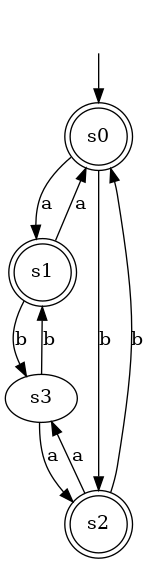
\includegraphics[width=0.2\linewidth]{images/dfa_even_a_or_even_b.png}
    \caption{Minimalny DFA dla języka $L$.}
    \label{fig:dfa_even_a_or_even_b}
\end{figure}

\paragraph*{Inicjalizacja tabeli obserwacji.}
Rozpoczynamy od tworzenia minimalnych zbiorów \textit{S} i \textit{E}:
\[
S = \{\epsilon\}, \quad E = \{\epsilon\}.
\]
Uczeń zadaje pytanie o członkostwo dla każdego elementu zbioru \( S \cup (S \cdot \Sigma) \):
\[
MQ(\epsilon) = 1, \quad MQ(a) = 1, \quad MQ(b) = 1.
\]
Wynik tego etapu można zobaczyć w tabeli \ref{tab:observation_1}. Jest ona \textbf{spójna} i \textbf{domknięta}. Można, więc skonstruować hipotezę.

\begin{table}
    \centering
    \begin{tabular}{c|c}
        \diagbox{\( S \cup (S \cdot \Sigma) \)}{$E$} & \( \epsilon \) \\
        \hline
        $\epsilon$      & 1 \\
        \hline
        $a$             & 1 \\
        $b$             & 1 \\
    \end{tabular}
    \caption{Początkowa tabela obserwacji.}
    \label{tab:observation_1}
\end{table}

\paragraph*{Konstrukcja hipotezy $H_1$.}
Na podstawie tabeli obserwacji \ref{tab:observation_1} konstruujemy hipotezę:
\begin{itemize}
    \item \textbf{Stany DFA:} \( q_\epsilon \), odpowiadający unikalnym wierszom tabeli.
    \item \textbf{Przejścia:}
    \begin{align*}
        & q_\epsilon \xrightarrow{a} q_\epsilon, \quad q_\epsilon \xrightarrow{b} q_\epsilon.
    \end{align*}
    \item \textbf{Stan początkowy:} \( q_\epsilon \).
    \item \textbf{Stany akceptujące:} \( q_\epsilon \).
\end{itemize}

\paragraph*{Testowanie hipotezy $H_1$.}
Hipoteza jest testowana przez zapytanie o równoważność ($EQ$). Można wybrać nieskończenie wiele kontrprzykładów, ale na potrzebę przykładu przyjmijmy, że nauczyciel zwraca $ba$.

\paragraph*{Aktualizacja tabeli obserwacji.}
Po otrzymaniu kontrprzykładu \( ba \), algorytm aktualizuje tabelę obserwacji. Wszystkie prefiksy \( ba \) są dodawane do zbioru \( S \), co prowadzi do:
\[
S = \{\epsilon, b, ba\}.
\]
Uczeń zadaje zapytania \( MQ \) dla nowych elementów \( S \cup (S \cdot \Sigma) \). Wyniki zapytań są następujące:
\[
MQ(ba) = 0, \quad MQ(baa) = 1, \quad MQ(bab) = 1.
\]
Wynikową tabelę obserwacji pokazano w tabeli \ref{tab:observation_2}. Jest ona \textbf{domknięta}, lecz \textbf{niespójna}, ponieważ:
\[
T(\epsilon, \epsilon) = T(b, \epsilon) \wedge T(\epsilon \cdot a, \epsilon) \neq T(b \cdot a, \epsilon),
\]
stąd $a$ jest rozróżniającym sufiksem. Dodajemy $a$ do $E$ i uzupełniamy tabelę obserwacji \ref{tab:observation_3}:
\[
MQ(\epsilon \cdot a) = 1, \quad MQ(b \cdot a) = 0, \quad MQ(ba \cdot a) = 1,
\]
\[
MQ(a \cdot a) = 1, \quad MQ(bb \cdot a) = 1, \quad MQ(baa \cdot a) = 0, \quad MQ(bab \cdot a) = 1.
\]
Tabela obserwacji jest teraz \textbf{domknięta} i \textbf{spójna}, więc możemy skonstruować hipotezę.

\begin{table}
    \centering
    \begin{tabular}{c|c}
        \diagbox{\( S \cup (S \cdot \Sigma) \)}{$E$} & \( \epsilon \) \\
        \hline
        $\epsilon$      & 1 \\
        $b$             & 1 \\
        $ba$            & 0 \\
        \hline
        $a$             & 1 \\
        $bb$            & 1 \\
        $baa$           & 1 \\
        $bab$           & 1 \\
    \end{tabular}
    \caption{Tabela obserwacji po otrzymaniu kontrprzykładu $ba$.}
    \label{tab:observation_2}
\end{table}

\begin{table}
    \centering
    \begin{tabular}{c|c|c}
        \diagbox{\( S \cup (S \cdot \Sigma) \)}{$E$} & \( \epsilon \) & $a$ \\
        \hline
        $\epsilon$      & 1 & 1 \\
        $b$             & 1 & 0 \\
        $ba$            & 0 & 1 \\
        \hline
        $a$             & 1 & 1 \\
        $bb$            & 1 & 1 \\
        $baa$           & 1 & 0 \\
        $bab$           & 1 & 1 \\
    \end{tabular}
    \caption{Tabela obserwacji po rozszerzeniu $E$ o element $a$.}
    \label{tab:observation_3}
\end{table}

\paragraph*{Konstrukcja hipotezy $H_2$.}
Na podstawie tabeli obserwacji \ref{tab:observation_3} konstruujemy hipotezę:
\begin{itemize}
    \item \textbf{Stany DFA:} \( q_\epsilon, q_b, q_{ba} \).
    \item \textbf{Przejścia:}
    \begin{align*}
        & q_\epsilon \xrightarrow{a} q_\epsilon, \quad q_\epsilon \xrightarrow{b} q_b, \\
        & q_b \xrightarrow{a} q_{ba}, \quad q_b \xrightarrow{b} q_\epsilon, \\
        & q_{ba} \xrightarrow{a} q_\epsilon, \quad q_{ba} \xrightarrow{b} q_b.
    \end{align*}
    \item \textbf{Stan początkowy:} \( q_\epsilon \).
    \item \textbf{Stany akceptujące:} \( q_\epsilon, q_b \).
\end{itemize}

\paragraph*{Testowanie hipotezy $H_2$.}
Hipoteza jest testowana przez zapytanie o równoważność ($EQ$). Ponownie można wybrać nieskończenie wiele kontrprzykładów. Przyjmijmy, więc, że nauczyciel zwraca $ab$.

\paragraph*{Aktualizacja tabeli obserwacji.}
Po otrzymaniu kontrprzykładu \( ab \), algorytm aktualizuje tabelę obserwacji. Na początek dodajemy \( a \) oraz \( ab \) do zbioru \( S \):
\[
S = \{ \epsilon, a, b, ab, ba \}.
\]
Uczeń zadaje pytania \( MQ \) dla nowych elementów zbioru \( S \cup (S \cdot \Sigma) \). Na tej podstawie aktualizujemy tabelę obserwacji. Wynikową tabelę obserwacji pokazano w tabeli \ref{tab:observation_4}. Tabela jest teraz \textbf{domknięta}, ale \textbf{niespójna}, ponieważ wiersz dla $\epsilon$ jest taki sam jak wiersz dla $a$, a wiersz dla \( \epsilon \cdot b \) jest inny niż wiersz dla \( a \cdot b \), stąd $b$ jest rozróżniającym sufiksem. Dodajemy $b$ do $E$ i uzupełniamy tabelę obserwacji \ref{tab:observation_5}. Dodanie \( b \) do \( E \) pozwala naprawić niespójność, rozróżniając zachowanie stanów dla różnych sufiksów.

\begin{table}
    \centering
    \begin{tabular}{c|c|c}
        \diagbox{\( S \cup (S \cdot \Sigma) \)}{$E$} & \( \epsilon \) & $a$ \\
        \hline
        $\epsilon$      & 1 & 1 \\
        $a$             & 1 & 1 \\
        $b$             & 1 & 0 \\
        $ab$            & 0 & 1 \\
        $ba$            & 0 & 1 \\
        \hline
        $aa$            & 1 & 1 \\
        $bb$            & 1 & 1 \\
        $aba$           & 1 & 0 \\
        $abb$           & 1 & 1 \\
        $baa$           & 1 & 0 \\
        $bab$           & 1 & 1 \\
    \end{tabular}
    \caption{Tabela obserwacji po dodaniu $a$ i $ab$ do $S$.}
    \label{tab:observation_4}
\end{table}

\begin{table}
    \centering
    \begin{tabular}{c|c|c|c}
        \diagbox{\( S \cup (S \cdot \Sigma) \)}{$E$} & $\epsilon$ & $a$ & $b$ \\
        \hline
        $\epsilon$      & 1 & 1 & 1 \\
        $a$             & 1 & 1 & 0 \\
        $b$             & 1 & 0 & 1 \\
        $ab$            & 0 & 1 & 1 \\
        $ba$            & 0 & 1 & 1 \\
        \hline
        $aa$            & 1 & 1 & 1 \\
        $bb$            & 1 & 1 & 1 \\
        $aba$           & 1 & 0 & 1 \\
        $abb$           & 1 & 1 & 0 \\
        $baa$           & 1 & 0 & 1 \\
        $bab$           & 1 & 1 & 0 \\
    \end{tabular}
    \caption{Tabela obserwacji po dodaniu $b$ do $E$.}
    \label{tab:observation_5}
\end{table}

\paragraph*{Konstrukcja hipotezy $H_3$.}
Na podstawie tabeli obserwacji konstruujemy hipotezę $H_3$:
\begin{itemize}
    \item \textbf{Stany DFA:} \( q_\epsilon, q_a, q_b, q_{ab} \), odpowiadające unikalnym wierszom tabeli.
    \item \textbf{Przejścia:}
    \begin{align*}
        & q_\epsilon \xrightarrow{a} q_a, \quad q_\epsilon \xrightarrow{b} q_b, \\
        & q_a \xrightarrow{a} q_\epsilon, \quad q_a \xrightarrow{b} q_{ab}, \\
        & q_b \xrightarrow{a} q_{ab}, \quad q_b \xrightarrow{b} q_\epsilon, \\
        & q_{ab} \xrightarrow{a} q_b, \quad q_{ab} \xrightarrow{b} q_a.
    \end{align*}
    \item \textbf{Stan początkowy:} \( q_\epsilon \).
    \item \textbf{Stany akceptujące:} \( q_\epsilon, q_a, q_b \), ponieważ odpowiadają sytuacjom, w których parzystość jednego z \( a \) lub \( b \) jest spełniona.
    \item \textbf{Stany nieakceptujące:} \( q_{ab} \), ponieważ odpowiada sytuacji, w której zarówno \( a \), jak i \( b \) mają nieparzystą liczbę wystąpień.
\end{itemize}

\paragraph*{Testowanie hipotezy $H_3$.}
Hipoteza jest testowana przez zapytanie o równoważność (EQ). Nauczyciel odpowiada ,,tak'', co kończy działanie algorytmu.

\paragraph*{Ostateczny automat.}
Automat DFA reprezentujący język \( L \) ma następującą macierz przejść:
\[
\begin{array}{c|c|c}
\text{Stan} & a & b \\
\hline
\rightarrow * q_\epsilon & q_a & q_b \\
* q_a & q_\epsilon & q_{ab} \\
* q_b & q_{ab} & q_\epsilon \\
q_{ab} & q_b & q_a \\
\end{array}
\]

\section{Algorytm \textit{RPNI}}
\label{sec:rpni}

\section{Algorytm \textit{GIG}}
\label{sec:gig}

Algorytm \textit{GIG} (\textit{Grammatical Inference by Genetic search}) \cite{GIG}, podobnie jak algorytm \textit{RPNI}, jest przeznaczony do indukcji gramatyk regularnych na podstawie przykładów pozytywnych \( S^+ \) i negatywnych \( S^- \). Oba algorytmy opierają się na iteracyjnym łączeniu stanów w celu skonstruowania deterministycznego automatu skończonego (DFA), który jak najlepiej opisuje dane. W przypadku \textit{RPNI} znaleziony DFA zawsze jest minimalny i akceptuje wszystkie słowa z \( S^+ \), odrzucając słowa z \( S^- \). Natomiast wynik algorytmu \textit{GIG} nie jest jednoznacznie określony.

W algorytmie \textit{GIG} przestrzeń możliwych rozwiązań jest reprezentowana jako podziały stanów maksymalnego automatu kanonicznego (MCA, ang. maximal canonical automaton) zbudowanego na podstawie zbioru \( S^+ \). Przeszukiwanie tej przestrzeni odbywa się przy użyciu algorytmu genetycznego, który iteracyjnie modyfikuje populację podziałów poprzez operacje takie jak krzyżowanie i mutacja. Funkcja dopasowania (\textit{fitness}) ocenia jakość każdego rozwiązania, preferując modele akceptujące jak najwięcej słów z \( S^+ \), odrzucające \( S^- \), a jednocześnie minimalizujące liczbę stanów. W efekcie uzyskane rozwiązanie może nie być optymalne ani w pełni poprawne.

W przeciwieństwie do deterministycznego podejścia algorytmu \textit{RPNI}, \textit{GIG} wykorzystuje mechanizmy ewolucyjne, co umożliwia efektywne przeszukiwanie dużych i złożonych przestrzeni rozwiązań. Jest to szczególnie istotne w przypadkach, gdy liczba stanów automatu lub rozmiar zbioru przykładów uczących znacząco rośnie.

W tej sekcji nie zostanie przedstawiony przykład działania, ponieważ jest to standardowy algorytm genetyczny. Zamiast tego, w podsekcji \ref{sec:gig-formalizacja} zostaną zaprezentowane przykłady operacji genetycznych, które pomogą zrozumieć działanie programu.

\subsection{Metoda}

GIG wykorzystuje algorytm genetyczny do indukcji deterministycznego automatu skończonego na podstawie przykładów pozytywnych i negatywnych. Kluczowym założeniem metody jest reprezentacja stanów maksymalnego automatu skończonego (MCA) jako podziału, który w procesie ewolucji jest optymalizowany pod kątem minimalizacji liczby stanów oraz zgodności z danymi wejściowymi.
\begin{enumerate}
    \item \textbf{Budowa automatu maksymalnego (MCA):}
        Na podstawie zbioru \( S^+ \) tworzony jest maksymalny automat skończony (MCA), w którym każdy stan odpowiada unikalnemu prefiksowi słów z \( S^+ \). MCA akceptuje dokładnie \( S^+ \), lecz nie jest minimalny.
    \item \textbf{Reprezentacja podziału stanów:}
        Stany MCA są reprezentowane jako podziały, gdzie każda grupa w podziale odpowiada jednemu stanowi w wynikowym DFA. Początkowa populacja składa się z losowych podziałów oraz rozwiązań opartych na strukturze MCA.
    \item \textbf{Ewolucja populacji:}
        Algorytm genetyczny iteracyjnie modyfikuje populację, stosując:
        \begin{itemize}
            \item \textbf{Krzyżowanie:} Łączenie dwóch podziałów w celu stworzenia nowych rozwiązań, przy zachowaniu strukturalnej zgodności podziałów.
            \item \textbf{Mutację:} Wprowadzanie losowych zmian w podziałach, aby eksplorować nowe obszary przestrzeni rozwiązań.
        \end{itemize}
    \item \textbf{Ocena dopasowania osobników (\textit{fitness}):}
        Każdy osobnik jest oceniany na podstawie skonstruowanego z niego DFA. Wartość dopasowania jest wyznaczana na podstawie liczby stanów DFA, zgodności z \( S^+ \) oraz zdolności do odrzucania \( S^- \). Preferowane są mniejsze automaty, które poprawnie klasyfikują dane.
    \item \textbf{Zakończenie:}
        Algorytm kończy działanie po osiągnięciu określonej liczby generacji lub spełnieniu kryterium stopu (np. brak poprawy w kolejnych iteracjach). Wynikowy podział definiuje DFA zgodny z \( S^+ \) i \( S^- \).
\end{enumerate}

\subsection{Różnice podejścia genetycznego i zachłannego}

Algorytm \textit{GIG} ma przewagę nad klasycznym algorytmem \textit{RPNI} w kontekście indukcji gramatyk regularnych, szczególnie w przypadku dużych i złożonych zestawów danych. Kluczową różnicą między oboma podejściami jest sposób przeszukiwania przestrzeni rozwiązań. \textit{RPNI} działa deterministycznie, łącząc stany automatu maksymalnego (PTA) w oparciu o reprezentatywność danych \( S^+ \) i \( S^- \), co pozwala na konstrukcję minimalnego automatu skończonego (DFA). Jednakże, w przypadku bardzo dużych przestrzeni rozwiązań algorytm deterministyczny może zawieść, nie będąc w stanie efektywnie eksplorować wszystkich możliwych podziałów.

W odróżnieniu od tego, \textit{GIG} wykorzystuje podejście ewolucyjne, co pozwala na bardziej elastyczne przeszukiwanie przestrzeni rozwiązań. Dzięki stochastycznemu charakterowi algorytmu genetycznego, \textit{GIG} jest w stanie znaleźć akceptowalne rozwiązanie, nawet jeśli nie jest ono optymalne. To podejście pozwala na radzenie sobie z ogromnymi zbiorami danych oraz sytuacjami, w których liczba stanów w automacie maksymalnym (MCA) znacząco wzrasta. Operacje genetyczne, takie jak krzyżowanie i mutacja, umożliwiają eksplorację przestrzeni podziałów w sposób mniej deterministyczny, zwiększając szansę na znalezienie rozwiązań w złożonych przypadkach.

Jednakże, w przeciwieństwie do deterministycznego podejścia \textit{RPNI}, algorytm \textit{GIG} nie gwarantuje, że uzyskane rozwiązanie będzie optymalne ani w pełni poprawne. Wynik może być jedynie przybliżeniem minimalnego automatu akceptującego \( S^+ \) i odrzucającego \( S^- \), co oznacza, że pewne nieścisłości w klasyfikacji mogą pozostać. Ponadto, czas działania \textit{GIG} jest uzależniony od parametrów takich jak liczba generacji i rozmiar populacji, co w niektórych przypadkach może prowadzić do wysokich kosztów obliczeniowych.

Dodatkowo, \textit{GIG} charakteryzuje się większą adaptacyjnością. Może dynamicznie dostosowywać populację oraz kryteria dopasowania (\textit{fitness}) do specyficznych cech problemu, co czyni go bardziej elastycznym w porównaniu do \textit{RPNI}. W sytuacjach, gdy przestrzeń stanów staje się zbyt duża dla deterministycznych podejść, \textit{GIG} potrafi efektywnie przeszukiwać tę przestrzeń dzięki heurystykom genetycznym, minimalizując ryzyko przeoczenia akceptowalnych rozwiązań.

Podsumowując, główną przewagą \textit{GIG} jest jego zdolność do radzenia sobie z ogromnymi zestawami danych oraz bardziej złożonymi strukturami języka, dzięki czemu może znaleźć rozwiązania, które są niedostępne dla deterministycznego podejścia \textit{RPNI}. Niemniej jednak, brak gwarancji optymalności i pełnej poprawności może być istotną wadą w sytuacjach wymagających precyzyjnych wyników.

\subsection{Formalizacja}
\label{sec:gig-formalizacja}

W tej sekcji opisano sposób przedstawienia rozwiązania w osobniku, proces inicjalizacji populacji, operatory genetyczne oraz funkcję przystosowania, która kieruje ewolucją. Dla każdego z tych elementów podano odpowiednie przykłady. Potrzebnymi definicjami dla tej sekcji będą definicja \ref{def:state_merging}, ponieważ łączenie stanów w \textit{GIG} przebiega w ten sam sposób co w \textit{RPNI}, oraz definicja \ref{def:pta}, jako że MCA w \textit{GIG} to dokładnie taka sama struktura co PTA w kontekście algorytmu \textit{RPNI}.

\paragraph*{Reprezentacja osobnika.}  
Każdy osobnik w populacji jest reprezentowany jako podział zbioru stanów \( Q \) automatu maksymalnego (MCA). Podział jest zakodowany jako wektor liczb całkowitych \( \mathbf{p} \), gdzie \( \mathbf{p}[i] = c \) oznacza, że stan \( q_i \in Q \) należy do grupy \( c \). Grupy odpowiadają stanom wynikowego deterministycznego automatu skończonego (DFA). Przykładowo, jeśli \( Q = \{q_0, q_1, q_2, q_3\} \), podział \( \mathbf{p} = [0, 0, 1, 1] \) oznacza, że stany \( q_0 \) i \( q_1 \) należą do jednej grupy, a \( q_2 \) i \( q_3 \) do drugiej.

Dla zapewnienia jednoznaczności i porównywalności osobników w populacji, podział \( \mathbf{p} \) musi być w formie kanonicznej. Oznacza to, że grupy w \( \mathbf{p} \) są ponumerowane w sposób ciągły, począwszy od \( 0 \), bez przeskoków w numeracji. Kanoniczność jest kluczowa, ponieważ pozwala unikać niejednoznaczności przy reprezentacji tego samego podziału oraz ułatwia operacje genetyczne, takie jak krzyżowanie i mutacja.

\textbf{Przykład:}  
Dla \( Q = \{q_0, q_1, q_2, q_3\} \), podział \( \mathbf{p} = [0, 2, 2, 5] \) nie jest kanoniczny, ponieważ grupy są ponumerowane z przeskokami (brakuje grup \( 1 \) i \( 3, 4 \)). Aby naprawić ten podział, każdej unikalnej wartości w \( \mathbf{p} \) przypisujemy nową numerację w kolejności ich występowania:
\[
\text{Niekanoniczny: } \mathbf{p} = [0, 2, 2, 5] \quad \rightarrow \quad \text{Kanoniczny: } \mathbf{p} = [0, 1, 1, 2].
\]

Naprawianie podziału jest procesem prostym, a dzięki kanonicznej formie reprezentacji różne osobniki o tej samej strukturze nie będą traktowane jako różne w trakcie ewolucji.

\paragraph*{Inicjalizacja populacji.}  
Początkowa populacja jest generowana w następujący sposób:
\begin{itemize}
    \item \textbf{Pierwszy osobnik:}  
    Pierwszy osobnik odpowiada obecnie rozszerzonemu automatowi (MCA), w którym każdy stan \( q_i \in Q \) należy do osobnej grupy. Przykładowo, dla \( Q = \{q_0, q_1, q_2, q_3\} \), pierwszy osobnik to \( \mathbf{p} = [0, 1, 2, 3] \).
    
    \item \textbf{Podziały z ograniczoną liczbą grup:}  
    Do 50\% populacji stanowią losowe podziały wybrane z \( \binom{|Q|}{2} \) możliwych podziałów, w których liczba grup wynosi \( |Q| - 1 \). Przykładowo, dla \( Q = \{q_0, q_1, q_2, q_3\} \), losowy podział może wyglądać tak: \( \mathbf{p} = [0, 0, 1, 2] \), gdzie \( q_0 \) i \( q_1 \) należą do tej samej grupy, a \( q_2 \) i \( q_3 \) są przypisane do osobnych grup.
    
    \item \textbf{Całkowicie losowe podziały:}  
    Pozostałe osobniki w populacji są generowane w sposób całkowicie losowy. Dla \( Q = \{q_0, q_1, q_2, q_3\} \), przykładowy losowy podział może wyglądać tak: \( \mathbf{p} = [0, 1, 1, 0] \), gdzie \( q_0 \) i \( q_3 \) należą do jednej grupy, a \( q_1 \) i \( q_2 \) do innej.
\end{itemize}

Takie podejście pozwala na inicjalizację populacji zarówno w oparciu o strukturalnie uzasadnione podziały, jak i bardziej eksploracyjne rozwiązania, zwiększając różnorodność przestrzeni początkowych rozwiązań.

\paragraph*{Mutacja.}  
Mutacja to operator genetyczny, który wprowadza losowe zmiany w reprezentacji osobnika \( \mathbf{p} \), pozwalając na eksplorację nowych podziałów przestrzeni rozwiązań. Formalnie, mutacja działa w następujący sposób:

Dla wybranego osobnika \( \mathbf{p} \), wybierany jest losowy indeks \( i \), gdzie 
\[ i \in \{0, 1, \dots, |Q|-1\}. \]

Wartość \( \mathbf{p}[i] \), odpowiadająca grupie przypisanej stanowi \( q_i \), jest zastępowana przez nową wartość \( c \), gdzie:
\[
c \in \{0, 1, \dots, \max(\mathbf{p}) + 1\}.
\]
Nowa wartość \( c \) może odpowiadać istniejącej grupie w \( \mathbf{p} \) lub utworzeniu nowej grupy. Po wykonaniu mutacji, wynikowy osobnik \( \mathbf{p}' \) jest kanonicznie porządkowany, aby zapewnić jednoznaczność reprezentacji.

\textbf{Przykład:}  
Dla osobnika \( \mathbf{p} = [0, 0, 1, 1] \), losowo wybrany indeks \( i = 3 \) (stan \( q_3 \)) prowadzi do zmiany wartości \( \mathbf{p}[3] \). Jeśli nowa wartość \( c \) to \( 2 \), to zmodyfikowany osobnik ma postać \( \mathbf{p}' = [0, 0, 1, 2] \). Po kanonicznej normalizacji osobnik pozostaje niezmieniony, ponieważ reprezentacja jest już poprawna.

\paragraph*{Krzyżowanie.}  
Krzyżowanie w algorytmie \textit{GIG} odbywa się w przestrzeni podziałów i polega na łączeniu wybranych bloków dwóch rodziców w celu utworzenia nowych osobników. Formalnie, dla dwóch rodziców \( \mathbf{p}_1 \) i \( \mathbf{p}_2 \), reprezentujących podziały \( \mathcal{P}_1 \) i \( \mathcal{P}_2 \), wybierane są losowe bloki \( B_1 \in \mathcal{P}_1 \) oraz \( B_2 \in \mathcal{P}_2 \). Bloki te są łączone w nowy blok \( B = B_1 \cup B_2 \), który zostaje wprowadzony do potomka. Nowy potomek dziedziczy pozostałe bloki od obojga rodziców, z uwzględnieniem połączenia. Po krzyżowaniu wynikowy podział jest normalizowany do postaci kanonicznej, aby zapewnić jednoznaczność reprezentacji osobnika.

\textbf{Przykład:}  
Dla dwóch rodziców:  
\[
\mathbf{p}_1 = [0, 0, 1, 1], \quad \mathbf{p}_2 = [0, 1, 1, 0],
\]
wybierane są bloki \( B_1 = \{q_0, q_1\} \) oraz \( B_2 = \{q_0, q_3\} \). Po połączeniu bloków \( B = B_1 \cup B_2 = \{q_0, q_1, q_3\} \), jeden z potomków może być reprezentowany jako:
\[
\mathbf{p} = [0, 0, 1, 0],
\]
gdzie \( q_0, q_1 \) i \( q_3 \) należą do jednej grupy, a \( q_2 \) do osobnej. Normalizacja potwierdza poprawność kanonicznej reprezentacji \( \mathbf{p} \).

\paragraph*{Funkcja przystosowania.}  
Funkcja przystosowania ocenia jakość osobników na podstawie poprawności ich podziału w kontekście danych \( S^+ \) i \( S^- \). Na przykład, DFA skonstruowany na podstawie osobnika \( \mathbf{p} = [0, 0, 1] \) może akceptować wszystkie słowa z \( S^+ \), ale odrzucać jedno słowo z \( S^- \), co obniża jego wartość przystosowania. Osobnik, który zarówno poprawnie akceptuje \( S^+ \), jak i odrzuca \( S^- \), uzyska wyższą wartość przystosowania.

\paragraph*{Proces ewolucji.}  
Algorytm iteracyjnie modyfikuje populację przez zastosowanie operatorów genetycznych (krzyżowanie i mutacja) oraz selekcję najlepszych osobników na podstawie funkcji przystosowania. Na przykład, w kolejnych generacjach populacja ewoluuje od początkowego rozwiązania \( \mathbf{p} = [0, 0, 1, 2] \) do \( \mathbf{p} = [0, 0, 0, 1] \), co prowadzi do uproszczonego automatu z mniejszą liczbą stanów.

\paragraph*{Wynik.}  
Rezultatem algorytmu jest DFA zminimalizowany na podstawie najlepszego osobnika końcowej populacji. Przykładowo, dla początkowego automatu MCA z czterema stanami \( Q = \{q_0, q_1, q_2, q_3\} \), wynikowy DFA może mieć tylko dwa stany, jeśli osobnik końcowy to \( \mathbf{p} = [0, 0, 1, 1] \).

\subsection{Złożoność}

W przypadku zastosowania algorytmu \textit{GIG} do indukcji gramatyk regularnych, złożoność czasowa zależy przede wszystkim od złożoności funkcji dopasowania i operatorów genetycznych, takich jak krzyżowanie i mutacja, które operują na podziałach stanów automatu maksymalnego (MCA). Liczba stanów \( Q \) w MCA oraz liczności zbiorów danych \( S^+ \) i \( S^- \) determinują koszt każdej generacji, ponieważ wpływają na czas potrzebny na konstrukcję automatu z danego podziału oraz sprawdzenie jego poprawności względem \( S^+ \) i \( S^- \).

W naszej konkretnej aplikacji nie mamy pewności, na ile wybrane operatory genetyczne oraz sposób kodowania problemu rzeczywiście oddają jego strukturę. Jest to kluczowa kwestia, ponieważ jakość dopasowania operatorów do problemu wpływa na tempo konwergencji algorytmu. Jeśli struktura problemu nie jest dobrze uchwycona przez funkcję dopasowania i operatory, algorytm może potrzebować więcej generacji, aby osiągnąć akceptowalne rozwiązanie. W praktyce nie jesteśmy w stanie przewidzieć, jak szybko algorytm będzie znajdował rozwiązania o wysokiej jakości, co sprawia, że jedynym sposobem na ocenę jego efektywności jest eksperymentalne testowanie dla różnych rozmiarów danych.

Zapotrzebowanie pamięciowe algorytmu wynika z przechowywania populacji, gdzie każdy osobnik jest reprezentowany jako podział zbioru \( Q \). Wymagana pamięć jest proporcjonalna do \( P \cdot |Q| \), gdzie \( P \) to liczba osobników w populacji. Dodatkowo, konieczne jest przechowywanie maksymalnego automatu skończonego (MCA), który wymaga \( O(|Q| \cdot |\Sigma|) \) pamięci, gdzie \( |\Sigma| \) to rozmiar alfabetu. Ponieważ automaty wynikowe są konstruowane dynamicznie podczas oceny funkcji dopasowania, a nie przechowywane dla każdego osobnika, pamięć nie jest dodatkowo obciążona przez pełne reprezentacje DFA.

Podsumowując, złożoność algorytmu \textit{GIG} w naszym przypadku jest determinowana głównie przez rozmiar zbiorów \( S^+ \), \( S^- \), liczbę stanów \( Q \), oraz zdolność operatorów genetycznych do odzwierciedlenia struktury problemu. Ze względu na brak pewności co do jakości tego dopasowania, ocena efektywności algorytmu wymaga praktycznych eksperymentów, które pozwolą lepiej zrozumieć jego zachowanie przy różnych rozmiarach danych.

\section{Algorytm \textit{ALERGIA}}  
\label{sec:alergia}  

Algorytm \textit{ALERGIA} \cite{ALERGIA} jest stosowany do indukcji stochastycznych gramatyk regularnych. W przeciwieństwie do \textit{RPNI} lub \textit{GIG}, które zakładają obecność zarówno przykładów pozytywnych, jak i negatywnych, \textit{ALERGIA} opiera się wyłącznie na zbiorze przykładów pozytywnych. Umożliwia to jego zastosowanie w sytuacjach, gdzie dostęp do przykładów negatywnych jest ograniczony lub niemożliwy.  

Algorytm ten konstruuje deterministyczny stochastyczny automat skończony (DSFA) na podstawie drzewa akceptacji prefiksów (PTA) utworzonego z dostępnych danych. Proces uogólniania polega na łączeniu stanów automatu, przy jednoczesnym zachowaniu zgodności ze statystycznym rozkładem prawdopodobieństwa przejść między stanami. Decyzje o scalaniu są podejmowane na podstawie testów statystycznych, które zapewniają, że wynikowy model zachowuje probabilistyczne własności danych wejściowych.  

Jedną z kluczowych cech algorytmu \textit{ALERGIA} jest jego zdolność do indukcji gramatyk stochastycznych, co czyni go szczególnie przydatnym w zastosowaniach wymagających modelowania niepewności lub probabilistycznych wzorców zachowań. Dzięki swojej efektywności obliczeniowej algorytm ten znajduje zastosowanie w zadaniach takich jak rozpoznawanie wzorców, analiza sekwencji biologicznych oraz modelowanie języka naturalnego.

Algorytm działa iteracyjnie, testując kompatybilność stanów i łącząc te, które są statystycznie zgodne. Proces kończy się, gdy żadne dalsze scalenie nie jest możliwe bez naruszenia kryteriów statystycznych. Dzięki temu wynikowy automat nie tylko reprezentuje język generowany przez dane treningowe, ale także umożliwia estymację prawdopodobieństwa generacji nowych ciągów.


\subsection{Metoda}  
Algorytm \textit{ALERGIA} pozwala na indukcję deterministycznego stochastycznego automatu skończonego (DSFA), który przybliża rozkład prawdopodobieństwa danych wejściowych. Proces ten obejmuje następujące kroki:  

\begin{enumerate}  
    \item \textbf{Budowa akceptora drzewa prefiksów (PTA):}  
        Zbiór przykładów pozytywnych jest używany do zbudowania deterministycznego automatu reprezentującego dokładnie wszystkie sekwencje w danych.  
    \item \textbf{Iteracyjne łączenie stanów:}  
        Algorytm analizuje pary stanów w PTA i testuje ich zgodność statystyczną. Łączenie stanów jest realizowane tylko wtedy, gdy nie narusza statystycznej zgodności z danymi.  
    \item \textbf{Sprawdzanie zgodności:}  
        Kompatybilność stanów jest oceniana za pomocą testu Hoeffding'a.  
    \item \textbf{Zakończenie:}  
        Algorytm kończy działanie, gdy żadne dalsze scalenie stanów nie jest możliwe bez naruszenia zgodności statystycznej. Ostateczny automat aproksymuje rozkład probabilistyczny danych wejściowych.  
\end{enumerate}


\subsection{Formalizacja}  
W tej sekcji przedstawiono matematyczne podstawy algorytmu \textit{ALERGIA} oraz definicje kluczowych pojęć, które umożliwiają precyzyjne opisanie jego działania. Algorytm ten wykorzystuje akceptor drzewa prefiksów (PTA) jako strukturę początkową z definicji \ref{def:pta}. Proces formalizacji skupia się na mechanizmach scalania stanów, które pozwalają na stopniowe upraszczanie automatu przy jednoczesnym zachowaniu zgodności z probabilistycznymi wzorcami danych wejściowych.  

\begin{definition}[DSFA]  
\label{def:dsfa}
Stochastyczny, skończony automat deterministyczny to piątka uporządkowana
\[ 
A = (Q, \Sigma, \delta, q_0, P), 
\]
gdzie:  
\begin{itemize}  
    \item \( Q \) – skończony zbiór stanów,  
    \item \( \Sigma \) – alfabet,  
    \item \( \delta : Q \times \Sigma \to Q \) – funkcja przejścia,  
    \item \( q_0 \in Q \) – stan początkowy,  
    \item \( P: Q \times \Sigma \to [0, 1] \) – funkcja prawdopodobieństwa przejść, spełniająca:  
    \[
    \sum_{a \in \Sigma} P(q, a) \leq 1, \quad \forall q \in Q, \quad a \in \Sigma.
    \]  
\end{itemize}
\end{definition}

Automat \( A \) generuje język stochastyczny, w którym każda sekwencja symboli z \( \Sigma \) jest akceptowana z określonym prawdopodobieństwem, wyznaczanym przez funkcję \( P \).

\begin{definition}[Test Hoeffding’a]  
\label{def:hoeffding_test}
Test Hoeffding’a w algorytmie ALERGIA jest wykorzystywany do porównania dwóch stanów \( q_1, q_2 \) poprzez wyznaczenie granicy tolerancji \( \epsilon \), która określa maksymalną dopuszczalną różnicę między ich rozkładami. Granica tolerancji \( \epsilon \) jest obliczana jako:  
\[
\epsilon = \sqrt{\frac{1}{2} \ln\left(\frac{2}{\alpha}\right)} \left( \frac{1}{\sqrt{n_1}} + \frac{1}{\sqrt{n_2}} \right),
\]
gdzie:  
\begin{itemize}  
    \item \( n_1, n_2 \) – liczba obserwacji w stanach \( q_1 \) i \( q_2 \),  
    \item \( \alpha \) – poziom ufności określający dopuszczalny margines błędu.  
\end{itemize}  
\end{definition}

Test Hoeffding’a to statystyczna metoda oceny zgodności dwóch rozkładów prawdopodobieństwa, bazująca na nierówności Hoeffding’a. W kontekście algorytmu \textit{ALERGIA} test ten służy do sprawdzania, czy różnice między obserwowanymi częstościami przejść w stanach automatu można uznać za przypadkowe, czy też są one statystycznie istotne. W algorytmie \textit{ALERGIA} test Hoeffding’a porównuje rozkłady przejść pomiędzy stanami automatu. Jeśli różnice są mniejsze niż wyznaczony próg tolerancji, stany są uznawane za zgodne statystycznie i mogą zostać scalone. 

\begin{definition}[Zgodność stanów]  
\label{def:alergia_state_compatibility}
Dwa stany \( q_1, q_2 \in Q \) są uznawane za zgodne (kompatybilne), jeżeli spełnione są dwa warunki:  
\begin{enumerate}
    \item Funkcja prawdopodobieństwa przejść \( P \) dla każdego symbolu \( a \in \Sigma \) spełnia:  
    \[
    |P(q_1, a) - P(q_2, a)| \leq \epsilon.
    \]  
    \item Prawdopodobieństwa terminacji \( P_F \) spełnia:
    \[
    |P_F(q_1) - P_F(q_2)| \leq \epsilon,
    \]  
    gdzie \( \epsilon \) jest granicą wyznaczoną przez test Hoeffding’a.
\end{enumerate}
\end{definition} 

\begin{definition}[Łączenie stanów w \textit{ALERGIA}]  
\label{def:alergia_state_merging}  
Łączenie dwóch stanów \( q_1, q_2 \in Q \) w stochastycznym, skończonym automacie deterministycznym (DSFA) \( A = (Q, \Sigma, \delta, q_0, P) \) polega na zintegrowaniu informacji o przejściach oraz rozkładach prawdopodobieństwa w jeden wspólny stan. Proces ten obejmuje następujące kroki:  

\begin{enumerate}  
    \item Wierzchołek reprezentujący stan \( q_2 \) zostaje przypisany jako poddrzewo do stanu \( q_1 \) poprzez modyfikację drzewa prefiksów.  
    \item Funkcja przejścia zostaje zaktualizowana:  
    \[
    \delta'(q, a) =
    \begin{cases}  
        \delta(q_1, a) & \text{jeśli } \delta(q, a) = q_2, \\  
        \delta(q, a) & \text{w przeciwnym przypadku.}  
    \end{cases}  
    \]  
    \item Przejścia oraz rozkłady prawdopodobieństwa dla symboli \( a \) są łączone poprzez uśrednienie wagowe:  
    \[
    P'(q, a) = \frac{n_1 \cdot P(q_1, a) + n_2 \cdot P(q_2, a)}{n_1 + n_2},
    \]  
    gdzie \( n_1 \) i \( n_2 \) oznaczają liczby obserwacji dla stanów \( q_1 \) i \( q_2 \).  
    \item Następnie wszystkie dzieci stanu \( q_2 \) zostają przeniesione do stanu \( q_1 \). Jeśli stan \( q_1 \) posiada już przejście dla danego symbolu, częstotliwości są sumowane. W przeciwnym przypadku tworzony jest nowy węzeł:  
    \[
    P'(q_1, a) = P(q_1, a) + P(q_2, a).
    \]  
    Proces ten jest kontynuowany rekurencyjnie dla wszystkich dzieci stanu \( q_2 \).  
\end{enumerate}  
\end{definition}  

Łączenie stanów jest przeprowadzane wyłącznie wtedy, gdy dwa stany oraz pary ich dzieci odpowiadające przejściom tych samych symboli spełniają kryteria zgodności określone w definicji \ref{def:alergia_state_compatibility}. Scalanie obejmuje także sumowanie obserwacji oraz prawdopodobieństw dla poddrzew, co zapewnia zachowanie struktury probabilistycznej danych wejściowych. Proces kończy się, gdy żadne dalsze połączenia nie spełniają warunków zgodności.  

% \subsection{Złożoność}  
% Algorytm \textit{ALERGIA} cechuje się złożonością wielomianową, zależną od rozmiaru danych wejściowych. W analizie złożoności czasowej i pamięciowej uwzględniamy następujące parametry:  
% \begin{itemize}  
%     \item \(|S^+|\) - liczba przykładów pozytywnych,  
%     \item \( l^+ \) - maksymalna długość ciągu w \( S^+ \),  
%     \item \(|Q|\) - liczba stanów w automacie,  
%     \item \(|\Sigma|\) - liczba symboli w alfabecie.  
% \end{itemize}  

% \paragraph*{Złożoność czasowa.}  
% Algorytm \textit{ALERGIA} składa się z dwóch głównych etapów: budowy drzewa prefiksowego oraz iteracyjnego scalania stanów.  

% \subparagraph*{Budowa drzewa prefiksowego (PTA).}  
% Pierwszy etap polega na utworzeniu drzewa prefiksowego (Prefix Tree Acceptor, PTA) na podstawie zbioru przykładów pozytywnych. Każde słowo jest dodawane do drzewa, a jego prefiksy są reprezentowane jako kolejne węzły. Proces ten wymaga analizy wszystkich przykładów oraz ich symboli, co prowadzi do złożoności:  
% \[
% O(|S^+| \cdot l^+).
% \]  

% \subparagraph*{Iteracyjne scalanie stanów.}  
% Drugi etap obejmuje iteracyjne porównywanie par stanów pod kątem zgodności, wykorzystując test Hoeffding’a. Każda para stanów jest sprawdzana pod względem zgodności prawdopodobieństw przejść i terminacji, a następnie wykonywane są rekurencyjne analizy następników. Sprawdzenie każdej pary stanów obejmuje:
% \begin{itemize}  
%     \item Porównanie prawdopodobieństw przejść dla wszystkich symboli w alfabecie \( \Sigma \).  
%     \item Rekurencyjne sprawdzenie zgodności następników.  
%     \item Ewentualne scalanie stanów, co wiąże się z aktualizacją przejść i prawdopodobieństw.  
% \end{itemize}  

% Złożoność iteracyjnego scalania stanów wynosi:  
% \[
% O(|Q|^4 \cdot |\Sigma|).
% \]  

% \subparagraph*{Złożoność rzeczywista.}  
% W praktyce rzeczywista złożoność algorytmu jest często znacznie niższa niż teoretyczna granica. Wynika to z dwóch głównych czynników:  
% \begin{enumerate}
%     \item Algorytm wcześnie scala zgodne stany, zmniejszając liczbę analizowanych stanów w kolejnych iteracjach.  
%     \item Stany znajdujące się na końcu porządku przetwarzania (liście drzewa) mają niewielu następców lub w ogóle ich nie posiadają, co ogranicza liczbę rekurencyjnych wywołań.  
% \end{enumerate}  

% Z tego powodu empiryczna złożoność algorytmu jest często bliższa:  
% \[
% O(|Q|^3 \cdot |\Sigma|).
% \]  

% \paragraph*{Łączna złożoność.}  
% Podsumowując, całkowita złożoność czasowa algorytmu obejmuje budowę drzewa oraz iteracyjne porównania i scalania stanów:  
% \[
% O(|S^+| \cdot l^+ + |Q|^4 \cdot |\Sigma|).
% \]

% \paragraph*{Zależność liczby stanów \( Q \).}  
% Liczba stanów \( |Q| \) w automacie jest bezpośrednio zależna od danych wejściowych. W najgorszym przypadku każde słowo o długości \( l^+ \) wnosi dokładnie \( l^+ \) nowych stanów. Przy \( |S^+| \) przykładach liczba stanów może wynosić:  
% \[
% |Q| \leq |S^+| \cdot l^+.
% \]  
% Z tego powodu rzeczywista złożoność algorytmu jest silnie powiązana z rozmiarem zbioru przykładów i długością słów.   
% \[
% O((|S^+| \cdot l^+)^4 \cdot |\Sigma|).
% \]


% \paragraph*{Złożoność pamięciowa}  
% Algorytm przechowuje następujące struktury:  
% \begin{itemize}  
%     \item \textbf{Drzewo prefiksowe (PTA):}  
%     PTA składa się z \( O(|S^+| \cdot l^+) \) stanów, z których każdy może mieć do \( |\Sigma| \) przejść. Wymagana przestrzeń pamięci wynosi:  
%     \[
%     O(|S^+| \cdot l^+ \cdot |\Sigma|).
%     \]  

%     \item \textbf{Statystyki przejść:}  
%     Dla każdego stanu przechowywane są rozkłady prawdopodobieństw oraz dane statystyczne, co daje dodatkowy koszt pamięciowy:  
%     \[
%     O(|S^+| \cdot l^+).
%     \]  
% \end{itemize}  

% Łączna złożoność pamięciowa wynosi:  
% \[
% O(|S^+| \cdot l^+ \cdot |\Sigma|).
% \]  

% \paragraph*{Czynniki wpływające na złożoność}  
% Efektywność algorytmu \textit{ALERGIA} zależy przede wszystkim od liczby przykładów pozytywnych (\( S^+ \)) oraz długości słów (\( l^+ \)), które determinują rozmiar drzewa prefiksowego i liczbę stanów do analizy. Dodatkowo, większy alfabet (\( |\Sigma| \)) zwiększa liczbę możliwych przejść, co wpływa zarówno na czas obliczeń, jak i wymagania pamięciowe.

\subsection{Przykład działania}  
Aby zilustrować działanie algorytmu \textit{ALERGIA}, rozważmy prosty przykład danych wejściowych opisujących sekwencje wyników rzutów monetą. Każdy wynik jest oznaczony symbolem \( H \) (orzeł) lub \( T \) (reszka).

\paragraph*{Dane wejściowe.}  
Zbiór przykładów pozytywnych (\( S^+ \)):  
\[
S^+ = \{H, H, T, HH, HT, TH, TT, HHH\}.
\]  

\paragraph*{Krok 1: Konstrukcja drzewa prefiksowego (PTA).}  
Na podstawie danych pozytywnych algorytm buduje drzewo prefiksowe (Prefix Tree Acceptor, PTA), które reprezentuje dokładnie wszystkie obserwowane sekwencje. Każdy stan odpowiada prefiksowi słów z \( S^+ \), a przejścia są etykietowane symbolami \( H \) lub \( T \). Wynik tego kroku można zobaczyć na rysunku \ref{fig:alergia_example_0}. 

\begin{figure}[ht]
    \centering
    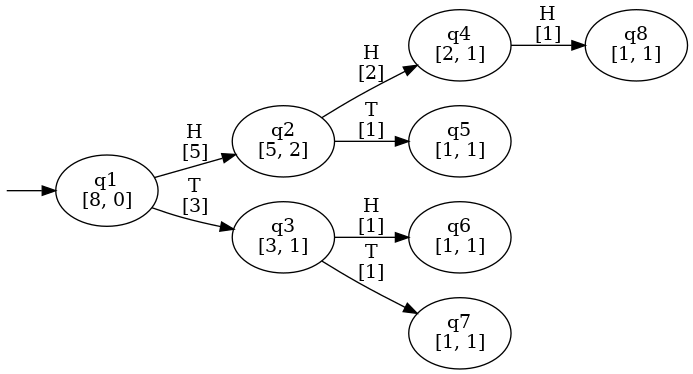
\includegraphics[width=0.8\textwidth]{images/run_example/alergia/0.png}
    \caption{Drzewo prefiksowe (PTA) skonstruowane dla \( S^+ \).}
    \label{fig:alergia_example_0}
\end{figure}

\paragraph*{Krok 2: Próba scalania stanów \( q_1 \) i \( q_2 \).}  
Algorytm rozpoczyna proces od analizy zgodności pierwszej pary stanów \( q_1 \) i \( q_2 \). Weryfikacja odbywa się na podstawie rozkładów prawdopodobieństw przejść oraz prawdopodobieństwa terminacji w obu stanach.  

\paragraph*{Dane stanów:}  
\begin{itemize}  
    \item \( q_1 \): \( n = 8, F = 0 \), przejścia: \( H[5], T[3] \).  
    \item \( q_2 \): \( n = 5, F = 2 \), przejścia: \( H[2], T[1] \).  
\end{itemize}  

\paragraph*{Sprawdzenie terminacji:}  
Prawdopodobieństwo terminacji dla każdego stanu:  
\[
P_F(q_1) = \frac{0}{8} = 0, \quad P_F(q_2) = \frac{2}{5} = \num{0.4},
\]

Różnica:  
\[
|P_F(q_1) - P_F(q_2)| = |0 - \num{0.4}| = \num{0.4}.
\]

\paragraph*{Tolerancja Hoeffding’a:}  
Przy poziomie ufności \( \alpha = \num{1.7} \) oraz liczbach obserwacji \( n_1 = 8 \) i \( n_2 = 5 \), granica zgodności \( \epsilon \) jest obliczana na podstawie wzoru:  
\[
\epsilon = \sqrt{\frac{\ln(2 / \alpha)}{2}} \left( \frac{1}{\sqrt{n_1}} + \frac{1}{\sqrt{n_2}} \right)
\]
\[
\epsilon \approx \num{0.228}.
\]

\paragraph*{Porównanie:}  
Ponieważ \( \num{0.4} > \num{0.228} \), stany \( q_1 \) i \( q_2 \) \textbf{nie mogą zostać połączone}.

\paragraph*{}

\paragraph*{Krok 3: Scalanie stanów \( q_2 \) i \( q_3 \).}  
Po odrzuceniu scalania stanów \( q_1 \) i \( q_2 \), algorytm przechodzi do analizy zgodności pary stanów \( q_2 \) i \( q_3 \).

\paragraph*{Dane stanów:}  
\begin{itemize}  
    \item \( q_2 \): \( n = 5, F = 2 \), przejścia: \( H[2], T[1] \), 
    \item \( q_3 \): \( n = 3, F = 1 \), przejścia: \( H[1], T[1] \).  
\end{itemize}  

\paragraph*{Test Hoeffding’a:}  
Prawdopodobieństwo terminacji dla każdego stanu:  
\[
P(q_2, H) = \frac{2}{5} = \num{0.4}, \quad P(q_3, H) = \frac{1}{3} \approx \num{0.333},
\]
\[
P(q_2, T) = \frac{1}{5} = \num{0.2}, \quad P(q_3, T) = \frac{1}{3} \approx \num{0.333},
\]
\[
P_F(q_2) = \frac{2}{5} = \num{0.4}, \quad P_F(q_3) = \frac{1}{3} \approx \num{0.333}.
\]

Różnica:  
\[
|P(q_2, H) - P(q_3, H)| \approx |\num{0.4} - \num{0.333}| = \num{0.067},
\]
\[
|P(q_2, T) - P(q_3, T)| \approx |\num{0.2} - \num{0.333}| = \num{0.133},
\]
\[
|P_F(q_2) - P_F(q_3)| \approx |\num{0.4} - \num{0.333}| = \num{0.067}.
\]

\paragraph*{Tolerancja Hoeffding’a:}  
Przy poziomie ufności \( \alpha = \num{1.7} \) oraz liczbach obserwacji \( n_1 = 5 \) i \( n_2 = 3 \), granica zgodności \( \epsilon \) jest obliczana na podstawie wzoru:  
\[
\epsilon = \sqrt{\frac{\ln(2 / \alpha)}{2}} \left( \frac{1}{\sqrt{n_1}} + \frac{1}{\sqrt{n_2}} \right)
\]
\[
\epsilon \approx \num{0.318}.
\]

\paragraph*{Porównanie:}  
Ponieważ:  
\[
|P(q_2, H) - P(q_3, H)| < \num{0.318}, \quad
\]
\[
|P(q_2, T) - P(q_3, T)| < \num{0.318}, \quad
\]
\[
|P_F(q_2) - P_F(q_3)| < \num{0.318},
\]  
stany \( q_2 \) i \( q_3 \) \textbf{są zgodne}. Aby mogły zostać połączone musimy sprawdzić rekurencyjnie zgodność dzieci stanu $q_3$ z odpowiednikami z gałęzi $q_2$, tj. $q_4$ i $q_6$ oraz $q_5$ i $q_7$. Analogiczne obliczenia wykazują zgodność wszystkich tych par stanów. Wynik tego kroku przedstawiono na rysunku \ref{fig:alergia_example_1}.  

\begin{figure}[ht]
    \centering
    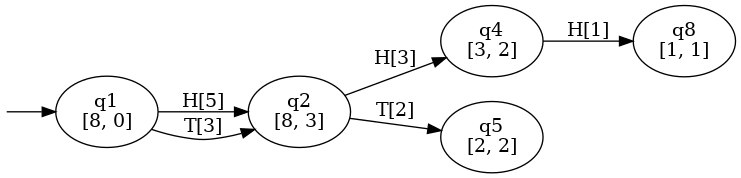
\includegraphics[width=0.8\textwidth]{images/run_example/alergia/1.png}
    \caption{Graf po scaleniu stanów \( q_2 \) i \( q_3 \).}
    \label{fig:alergia_example_1}
\end{figure}

\paragraph*{Krok 4: Scalanie stanów \( q_4 \) i \( q_8 \).}  
Po wcześniejszym scaleniu stanów \( q_2 \) i \( q_3 \), \( q_4 \) i \( q_6 \) oraz \( q_5 \) i \( q_7 \), algorytm przechodzi do następnej zgodnej pary stanów \( q_4 \) i \( q_8 \). Stan \( q_4 \) po wcześniejszym scaleniu z \( q_6 \) posiada \( n = 3, F = 2 \) oraz przejście \( H[1] \). Stan \( q_8 \) ma \( n = 1, F = 1 \) i brak przejść. Obliczenia są przeprowadzane analogicznie do wcześniejszych kroków. Porównanie prawdopodobieństw przejść oraz terminacji pokazuje, że różnice mieszczą się w zakresie tolerancji Hoeffding’a. Dzięki temu stany mogą zostać połączone, tworząc nowy stan \( q_4 \) o wartościach \( n = 4, F = 3 \) oraz przejściem zwrotnym \( H[1] \). Wynik tego kroku przedstawiono na rysunku \ref{fig:alergia_example_2}.  

\begin{figure}[ht]
    \centering
    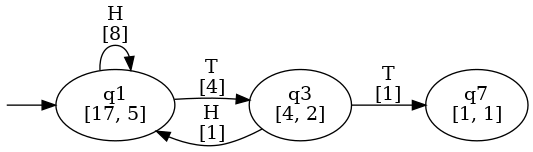
\includegraphics[width=0.8\textwidth]{images/run_example/alergia/2.png}
    \caption{Graf po scaleniu stanów \( q_4 \) i \( q_8 \).}
    \label{fig:alergia_example_2}
\end{figure}  

\paragraph*{Krok 5: Scalanie stanów \( q_4 \) i \( q_5 \).}  
Po wcześniejszych krokach, w których scalono stany \( q_2 \) z \( q_3 \), \( q_4 \) z \( q_6 \) oraz \( q_5 \) z \( q_7 \), algorytm przechodzi do analizy zgodności pary stanów \( q_4 \) i \( q_5 \). Stan \( q_4 \) po wcześniejszych operacjach posiada \( n = 3, F = 2 \) z przejściem zwrotnym \( H[1] \), natomiast stan \( q_5 \) ma \( n = 2, F = 2 \) i brak przejść. Obliczenia Hoeffding’a przeprowadzone w sposób analogiczny do wcześniejszych kroków pokazują, że różnice w rozkładach prawdopodobieństw przejść oraz terminacji mieszczą się w zakresie tolerancji. Dzięki temu stany zostają połączone, tworząc nowy stan \( q_4 \) z wartościami \( n = 5, F = 4 \) oraz przejściem zwrotnym \( H[1] \). Wynikowy graf można zobaczyć na rysunku \ref{fig:alergia_example_3}.

\begin{figure}[ht]
    \centering
    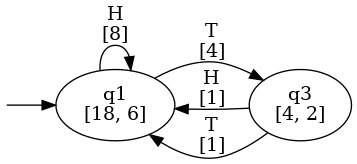
\includegraphics[width=0.8\textwidth]{images/run_example/alergia/3.png}
    \caption{Graf po scaleniu stanów \( q_4 \) i \( q_5 \).}
    \label{fig:alergia_example_3}
\end{figure}  

\paragraph*{Przekształcenie do postaci probabilistycznej.}  
W ostatnim kroku przekształcamy graf do postaci probabilistycznej. Prawdopodobieństwa terminacji oraz przejść są obliczane w sposób analogiczny do poprzednich kroków, uwzględniając wartości dla każdego stanu oraz przejść między nimi. Finalna postać grafu probabilistycznego reprezentuje rozkład danych wejściowych i umożliwia estymację nowych sekwencji. Wynikowy automat stochastyczny odwzorowuje prawdopodobieństwa przejść oraz terminacji, zapewniając zgodność probabilistyczną z danymi treningowymi. Wyniki tych kroków przedstawiono na rysunkach \ref{fig:alergia_example_4}.  

\begin{figure}[ht]
    \centering
    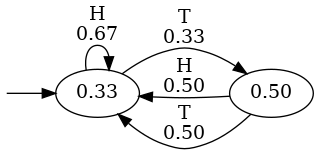
\includegraphics[width=0.8\textwidth]{images/run_example/alergia/4.png}
    \caption{Graf z probabilistycznymi przejściami i terminacjami.}
    \label{fig:alergia_example_4}
\end{figure}  

\paragraph*{Podsumowanie:}  
Algorytm zakończył proces scalania, redukując liczbę stanów i upraszczając strukturę automatu. Wynikowy automat stochastyczny zachowuje zgodność probabilistyczną z danymi wejściowymi, reprezentując ich rozkłady prawdopodobieństwa w sposób bardziej uogólniony. Finalna postać automatu pozwala na estymację nowych sekwencji zgodnych z rozkładem danych treningowych.  


    \chapter{Eksperymenty}
\label{cha:eksperymenty}

% Mimo swoich zalet, \textit{ALERGIA} zazwyczaj nie jest odpowiednim wyborem do zastąpienia algorytmów \textit{GIG}, \textit{RPNI} lub \textit{L*}. Algorytm zakłada wyłącznie przykłady pozytywne, co ogranicza jego zdolność do wykrywania granic języka i może prowadzić do zbyt ogólnych modeli. Algorytmy takie jak \textit{RPNI} uwzględniają także przykłady negatywne, co pozwala na precyzyjniejsze modelowanie. Ponadto, \textit{ALERGIA} jest zoptymalizowana pod kątem modeli probabilistycznych, co czyni go mniej odpowiednim w przypadkach, gdzie wymagane są deterministyczne gramatyki lub klasyczne modele bez prawdopodobieństw, jak \textit{GIG} i \textit{L*}. Dlatego \textit{ALERGIA} sprawdza się głównie w zadaniach probabilistycznych, gdzie brak przykładów negatywnych, natomiast w kontekście klasycznych gramatyk regularnych bardziej odpowiednie pozostają algorytmy \textit{GIG}, \textit{RPNI} i \textit{L*}.

% Celem przeprowadzonych eksperymentów jest analiza zachowania wybranych algorytmów indukcji gramatyk formalnych w różnych warunkach oraz ocena ich wydajności, dokładności i odporności na zmiany parametrów. Badaniom poddano cztery algorytmy: \textit{RPNI}, \textit{L*}, \textit{ALERGIA} oraz \textit{GIG}. Eksperymenty opierają się na danych syntetycznych, które zostały dobrane indywidualnie pod kątem specyfiki każdego testowanego algorytmu. Dane zostały przygotowane tak, aby umożliwić ocenę złożoności czasowej, liczby stanów wynikowych automatów oraz zdolności do generalizacji na podstawie przykładów treningowych.  

Algorytm \textit{RPNI} poddano analizie pod względem złożoności czasowej oraz dokładności modelu w zależności od rozmiaru alfabetu. Metryki użyte do oceny obejmują czas działania algorytmu oraz liczbę stanów wynikowego automatu. W przypadku algorytmu \textit{L*} skupiono się na liczbie zapytań EQ (\textit{Equivalence Query}) i MQ (\textit{Membership Query}) w zależności od złożoności problemu. Zebrane dane obejmują liczbę zapytań EQ i MQ oraz rozmiar wynikowego automatu. Dla algorytmu \textit{ALERGIA} przeprowadzono testy odporności na szum w danych, analizując procent poprawnie wygenerowanych zdań spośród \( N \) przykładów oraz liczbę stanów w automacie wynikowym. Z kolei algorytm \textit{GIG} poddano analizie pod kątem wpływu populacji początkowej na jego dokładność i wydajność. Wyniki oceniono na podstawie czasu działania, liczby generacji, liczby stanów automatu oraz procentu poprawnych klasyfikacji danych testowych.


\section{Eksperymenty dla algorytmu \textit{L*}}
Eksperymenty przeprowadzone dla algorytmu \textit{L*} mają na celu analizę liczby zapytań oraz rozmiaru wynikowego automatu w zależności od złożoności problemu. Badania obejmują dwa przypadki testowe, z których każdy analizuje inną klasę języków formalnych. W obu eksperymentach przyjęto alfabet \(\{0, 1\}\). 
W eksperymentach nie powtarzano testów, ponieważ algorytm \textit{L*} działa w sposób deterministyczny, a jego wynik zależy wyłącznie od dostarczonych danych wejściowych oraz użytego źródła wiedzy (\textit{oracle}). Wykorzystana w badaniach wyrocznia jest deterministyczna, gdyż opiera się na wcześniej utworzonym deterministycznym automacie skończonym (DFA). Oznacza to, że odpowiada na każde zapytanie zgodnie z definicją języka i nie wprowadza niepewności ani błędów. W związku z tym algorytm zawsze generuje ten sam wynik dla tych samych parametrów, co eliminuje potrzebę wielokrotnego wykonywania testów w celu uśrednienia wyników.

\subsection{Eksperyment 1: Język z prefiksem zer}
\label{sec:eksperyment1}

Pierwszy eksperyment bada język opisany wyrażeniem regularnym:  
\[
L_n = 0^n(0 \cup 1)^*,
\]  
gdzie \( n \) określa liczbę zer występujących na początku ciągu, a następnie mogą pojawiać się dowolne symbole z alfabetu \(\{0, 1\}\). Język ten opisuje wzorce o stałym prefiksie zer, które mogą być dowolnie kontynuowane. Badane są wartości \( n \) w zakresie od 1 do 64. Przykładowo, dla \( n = 2 \) język obejmuje ciągi takie jak:  
\[
L_2 = \{00, 000, 001, 0010, 0011, \ldots \}.
\]  

\subsection{Eksperyment 2: Język z równoważnymi blokami} 
\label{sec:eksperyment2}

Eksperyment bada język zdefiniowany jako:  
\[
L_n = \bigcup_{m=1}^{n} 0^m 1^m(0 + 1)^*,
\]  
gdzie \( n \) określa maksymalną liczbę powtórzeń symboli \( 0 \) i \( 1 \) w blokach symetrycznych, po których mogą następować dowolne symbole z alfabetu \(\{0, 1\}\). Język ten opisuje wzorce o równoważnych blokach zer i jedynek, które mogą stanowić prefiks dłuższego ciągu. Badany zakres wartości parametru \( n \) wynosi od 1 do 9. Przykładowo, dla \( n = 2 \) język obejmuje ciągi:  
\[
L_2 = \{01, 0011, 00110, 001101, 0011010111, \ldots\}.
\]

\subsection{Metryki oceny}  
W trakcie eksperymentów analizowane są następujące metryki:  
\begin{itemize}  
    \item Liczba zapytań o równoważność (\textit{EQ}),  
    \item Liczba zapytań o przynależność (\textit{MQ}),  
    \item Liczba stanów w wynikowym automacie.
\end{itemize}  

Liczba zapytań \textit{EQ} oraz \textit{MQ} pozwala ocenić efektywność algorytmu pod względem liczby interakcji wymaganych do nauki modelu. Liczba stanów w wynikowym automacie służy do oceny zdolności algorytmu do odwzorowania struktury badanego języka przy jednoczesnym minimalizowaniu jego złożoności.  

\subsection{Procedura eksperymentów}  
Każda konfiguracja parametrów jest analizowana pojedynczo, ponieważ algorytm działa w sposób deterministyczny, co oznacza, że wyniki są powtarzalne dla tych samych danych wejściowych. Dzięki temu nie ma potrzeby wielokrotnego wykonywania testów w celu uśrednienia wyników.  


\section{Eksperyment dla algorytmu \textit{RPNI}}  
Eksperymenty przeprowadzone dla algorytmu \textit{RPNI} mają na celu analizę wpływu rozmiaru alfabetu na złożoność czasową oraz strukturę wynikowego automatu. Badany język składa się ze wszystkich ciągów rozpoczynających się symbolem \( 0 \), po którym mogą występować dowolne symbole z przyjętego alfabetu. Formalnie język można opisać wyrażeniem regularnym:  
\[
L = 0(0 + 1 + \ldots + k)^*,
\]  
gdzie \( k \) określa maksymalny symbol w danym alfabecie.  

Przykładowo, dla alfabetu \(\{0, 1\}\) język obejmuje ciągi:  
\[
L = \{0, 01, 00, 010, 0111, 00101, \ldots \}.
\]  

Dane testowe są generowane w taki sposób, aby jednoznacznie opisywały język. Liczba przykładów oraz długości sekwencji są dobierane empirycznie, aby zapewnić porównywalną złożoność obliczeniową dla każdego rozmiaru alfabetu. Eksperyment bada wpływ rozmiaru alfabetu na działanie algorytmu. Testowane wartości wielkości alfabetu to:  
\[
|\Sigma| = \{2, 4, 8, 16, 32, 64\}.
\]  
Dla każdej wartości alfabetu dane są dynamicznie generowane, a następnie analizowane przez algorytm.  
\subsection{Metryki oceny}  
W trakcie eksperymentu analizowane są następujące metryki:  
\begin{itemize}  
    \item Liczba stanów w wynikowym automacie,  
    \item Czas wykonania algorytmu.  
\end{itemize}  

Liczba stanów w wynikowym automacie służy do oceny zdolności algorytmu do poprawnego uogólniania danych wejściowych.  

\subsection{Procedura eksperymentu}  
Każda konfiguracja parametrów jest testowana 50 razy, a uzyskane wartości są uśredniane w celu zminimalizowania wpływu zmienności danych na pomiary. Eksperymenty są przeprowadzane w sposób deterministyczny, co oznacza, że wyniki dla danej konfiguracji parametrów są powtarzalne.  


\section{Eksperymenty dla algorytmu \textit{GIG}} 
Eksperymenty przeprowadzone dla algorytmu \textit{GIG} mają na celu analizę wpływu sposobu inicjalizacji populacji początkowej na jakość wynikowego automatu oraz liczbę generacji potrzebnych do znalezienia rozwiązania. Eksperyment bada dwa podejścia do inicjalizacji populacji początkowej:  
\begin{itemize}  
    \item Losowa populacja -- generowana całkowicie losowo.  
    \item Inteligentna populacja -- skonstruowana tak jak zostało to opisane w sekcji \ref{sec:gig-formalizacja}.  
\end{itemize}  

Parametry algorytmu, takie jak liczba generacji (\(2000\)), liczba rodziców (\(20\)) oraz rozmiar populacji (\(100\)), pozostają stałe we wszystkich testach. Kryterium zatrzymania obejmuje warunek, który kończy proces po 50 generacjach bez poprawy jakości rozwiązania. W eksperymencie wykorzystano trzy różne języki formalne, dla których zdefiniowano zbiory przykładów pozytywnych i negatywnych. 

\subsection{Język 1: Co najmniej jedno \( a \)}  
\label{sec:eksperyment4}
Język ten obejmuje wszystkie ciągi zawierające przynajmniej jeden symbol \( a \).  
\begin{itemize}  
    \item Przykłady pozytywne: \( \epsilon, a, aa, ab, ba, aba, aab, baa, abaaa, baaaa, ac, ca, aca, cac, cacac \).  
    \item Przykłady negatywne: \( b, bb, c, bc, bbb, bbb, bbbc \).  
\end{itemize}  

\subsection{Język 2: Parzysta liczba \( a \) lub \( b \)}  
\label{sec:eksperyment5}
Język ten akceptuje ciągi, w których liczba symboli \( a \) lub \( b \) jest parzysta.  
\begin{itemize}  
    \item Przykłady pozytywne: \( \epsilon, a, b, aa, bb, abb, aab, baa, aba, abaaa, baaaa \).  
    \item Przykłady negatywne: \( ab, ba, aaab, aaba, abaa, baaa, abbb, bbba, ababab \).  
\end{itemize}  

\subsection{Język 3: Parzysta liczba \( a \)}  
\label{sec:eksperyment6}
Język ten obejmuje wszystkie ciągi, w których liczba symboli \( a \) jest parzysta.  
\begin{itemize}  
    \item Przykłady pozytywne: \( \epsilon, b, aa, aab, bb, baa, aba, abaaa, baaaa \).  
    \item Przykłady negatywne: \( a, ab, ba, aaa, aaba, abb, ababab \).  
\end{itemize}

\subsection{Metryki oceny}  
W trakcie eksperymentów analizowane są następujące metryki:  
\begin{itemize}
    \item Numer pokolenia najlepszego rozwiązania -- liczba opisująca w ilu cyklach algorytm genetyczny znalazł rozwiązanie.
    \item Jakość -- procent poprawnych klasyfikacji najlepszego osobnika na danych testowych.
    \item Macierz konfuzji -- cztery wartości opisujące ilość błędów najlepszego osobnika.
\end{itemize}  

\subsection{Procedura eksperymentów}  
Każda konfiguracja inicjalizacji populacji jest testowana 50 razy dla każdego z języków formalnych, a uzyskane wartości są uśredniane. Eksperymenty są przeprowadzane na wszystkich danych wejściowych, co umożliwia porównanie wydajności algorytmu w zależności od struktury danych i sposobu inicjalizacji populacji.  


\section{Eksperyment dla algorytmu \textit{ALERGIA}}  
Eksperyment przeprowadzony dla algorytmu \textit{ALERGIA} ma na celu analizę jego odporności na szum w danych wejściowych. Algorytm testowany jest pod kątem jakości wygenerowanego modelu oraz liczby stanów wynikowego automatu w zależności od poziomu zakłóceń. Badany język składa się z ciągów naprzemiennych symboli \( a \) i \( b \). Formalnie język można opisać wyrażeniem regularnym:  
\[
L = (ab)^* a?,
\]  
gdzie symbol \( ? \) oznacza, że pojedyncze \( a \) może, ale nie musi, wystąpić na końcu.  

Przykładowe ciągi należące do języka to:  
\[
\{a, ab, aba, abab, ababa, abababab, \ldots\}.
\]  

Zbiór danych testowych zawiera 1000 przykładów pozytywnych oraz 1000 przykładów negatywnych. Przykłady negatywne są generowane losowo z automatu komplementarnego do badanego języka. Automat ten akceptuje wszystkie ciągi, które nie należą do języka naprzemiennych symboli \( a \) i \( b \). Dzięki temu przykłady negatywne obejmują zarówno strukturalnie błędne ciągi (np. \( abb \), \( baa \)), jak i losowe permutacje symboli spoza badanego języka. Eksperyment bada wpływ poziomu szumu w danych na jakość wynikowego modelu. Szum jest dodawany do danych w stosunku, który przyjmuje wartości:  
\[
\{\num{0.0}, \num{0.001}, \num{0.005}, \num{0.01}, \num{0.02}, \num{0.05}, \num{0.1}, \num{0.2}, \num{0.3}, \num{0.4}, \num{0.5}\}.
\]  
Każdy zestaw danych z określonym poziomem zakłóceń jest analizowany niezależnie.  

\subsection{Metryki oceny}  
W trakcie eksperymentu analizowane są następujące metryki:  
\begin{itemize}  
    \item Jakość modelu -- procent poprawnych zdań wygenerowanych przez automat spośród \num{10000} losowo wygenerowanych prób.  
    \item Liczba stanów w wynikowym automacie.  
\end{itemize}  

Jakość modelu jest mierzona przez symulację jego działania na losowo wygenerowanych ciągach. Automat uznaje ciąg za poprawny, jeśli spełnia on warunki języka naprzemiennych symboli \( a \) i \( b \).  

\subsection{Procedura eksperymentu}  
Każda konfiguracja poziomu szumu jest testowana 50 razy, a uzyskane wartości są uśredniane. Eksperymenty są przeprowadzane dla wszystkich poziomów zakłóceń w celu analizy wpływu szumu na zdolność algorytmu do odwzorowania struktury badanego języka.  


\section{Kod źródłowy i odtwarzanie eksperymentów}  
\label{sec:code}  

Wszystkie eksperymenty opisane w pracy zostały zaimplementowane i udostępnione w publicznym repozytorium\footnote{\url{https://github.com/pepe5p/grammar-induction}}. Repozytorium zawiera kod źródłowy, dane testowe oraz szczegółowe instrukcje umożliwiające odtworzenie eksperymentów. Aby uruchomić eksperymenty, należy wykonać następujące kroki:  
\begin{itemize}  
    \item Upewnić się, że \textit{Docker} oraz \textit{Docker Compose} są zainstalowane w systemie.  
    \item Sklonować repozytorium i przejść do jego katalogu. Przykładowe polecenia:  
    \begin{minted}{bash}
    git clone https://github.com/pepe5p/grammar-induction
    cd grammar-induction
    \end{minted} 
    \item Zbudować obraz Dockerowy, wykonując polecenie:  
    \begin{minted}{bash}
    docker compose build grammar-induction
    \end{minted}  
    \item Uruchomić eksperyment za pomocą polecenia:  
    \begin{minted}{bash}
    make dc_run
    \end{minted}
    Po wywołaniu polecenia należy podać nazwę algorytmu, np.\ ,,\texttt{alergia}''.
\end{itemize} 

Aby zmienić parametry testów, należy edytować kod źródłowy repozytorium.

    \chapter{Wyniki i wnioski}  
\label{cha:wyniki}  

W tym rozdziale przedstawiono wyniki i wnioski z eksperymentów przeprowadzonych dla algorytmów \textit{L*}, \textit{RPNI}, \textit{GIG} oraz \textit{ALERGIA}. Celem eksperymentów była analiza skuteczności, wydajności oraz zdolności do uogólniania danych przez każdą z metod. Tabele i wykresy ilustrują zależności między parametrami wejściowymi a metrykami, takimi jak liczba stanów w automatach, liczba zapytań oraz czas wykonania. Każdy algorytm testowano na odpowiednio dobranych danych, aby uwzględnić jego specyficzne właściwości i ograniczenia.


\section{Algorytm \textit{L*}}  
W tej sekcji przedstawiono wyniki eksperymentów przeprowadzonych dla algorytmu \textit{L*}. Analizowano liczbę zapytań oraz rozmiar wynikowego automatu w zależności od złożoności problemu. 

Tabele \ref{tab:lstar_prefix} oraz \ref{tab:lstar_blocks} przedstawiają wyniki eksperymentów. Kolumna \textit{Rozmiar problemu (\(n\))} określa poziom złożoności testowanego języka. Kolumny \textit{EQ} oraz \textit{MQ} zawierają odpowiednio liczbę zapytań o równoważność hipotez oraz przynależność, które były wymagane do skonstruowania poprawnego modelu. Ostatnia kolumna, \textit{Rozmiar DFA}, wskazuje liczbę stanów w wynikowym automacie deterministycznym (\textit{DFA}).

Jak pokazano na wykresie \ref{fig:lstar_prefix_mq}, liczba zapytań o przynależność (\textit{MQ}) rośnie wykładniczo wraz ze wzrostem rozmiaru problemu (\(n\)). Liczba zapytań o równoważność (\textit{EQ}) pozostaje natomiast niewielka, co sugeruje, że algorytm efektywnie formułuje hipotezy dotyczące struktury języka. Rozmiar wynikowego automatu (\textit{DFA}) rośnie liniowo w stosunku do złożoności problemu, co potwierdza zdolność algorytmu do uogólniania danych przy zachowaniu minimalnej liczby stanów. Wyniki pokrywają się z liczbą stanów minimalnego automatu, opisaną wzorem \( n + 2 \).

Wyniki przedstawione na wykresie \ref{fig:lstar_blocks_mq} również wskazują wykładniczy wzrost liczby zapytań (\textit{MQ}) wraz z rozmiarem problemu. W tym przypadku odnotowano większą liczbę zapytań o równoważność (\textit{EQ}) w porównaniu do poprzedniego eksperymentu, co sugeruje, że algorytm wymaga więcej prób do rozpoznania bardziej złożonych wzorców. Liczba zapytań o równoważność zależy od specyfiki problemu i może być trudna do przewidzenia. Rozmiar automatu (\textit{DFA}) rośnie liniowo, co potwierdza minimalność modelu, zgodnie ze wzorem \( 2n + 2 \).

\begin{table}[h]
\centering
\caption{Wyniki eksperymentu z sekcji \ref{sec:eksperyment1}.}
\label{tab:lstar_prefix}
\begin{tabular}{|c|c|c|c|}
\hline
Rozmiar problemu (\(n\)) & EQ & MQ & Rozmiar DFA \\ \hline
1                        & 2  & 13 & 3           \\ \hline
2                        & 3  & 25 & 4           \\ \hline
4                        & 3  & 61 & 6           \\ \hline
8                        & 3  & 181 & 10         \\ \hline
16                       & 3  & 613 & 18         \\ \hline
32                       & 3  & 2245 & 34        \\ \hline
64                       & 3  & 8581 & 66        \\ \hline
\end{tabular}
\end{table}

\begin{figure}[h]
\centering
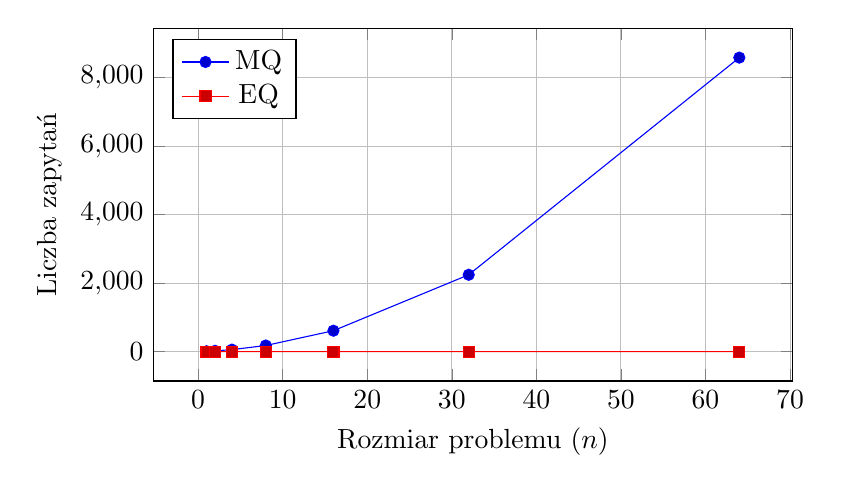
\begin{tikzpicture}
\begin{axis}[
    xlabel={Rozmiar problemu (\(n\))},
    ylabel={Liczba zapytań},
    legend pos=north west,
    grid=major,
    width=0.8\textwidth,
    height=0.5\textwidth
]

% MQ
\addplot coordinates {(1, 13) (2, 25) (4, 61) (8, 181) (16, 613) (32, 2245) (64, 8581)};
\addlegendentry{MQ}

% EQ
\addplot coordinates {(1, 2) (2, 3) (4, 3) (8, 3) (16, 3) (32, 3) (64, 3)};
\addlegendentry{EQ}

\end{axis}
\end{tikzpicture}
\caption{Zależność liczby zapytań EQ i MQ od rozmiaru problemu dla języka z sekcji \ref{sec:eksperyment1}.}
\label{fig:lstar_prefix_mq}
\end{figure}

\begin{table}[h]
\centering
\caption{Wyniki eksperymentu z sekcji \ref{sec:eksperyment2}.}
\label{tab:lstar_blocks}
\begin{tabular}{|c|c|c|c|}
\hline
Rozmiar problemu (\(n\)) & EQ & MQ & Rozmiar DFA \\ \hline
1                        & 3  & 24  & 4           \\ \hline
2                        & 4  & 54  & 6           \\ \hline
3                        & 5  & 104 & 8           \\ \hline
4                        & 6  & 180 & 10          \\ \hline
5                        & 7  & 288 & 12          \\ \hline
6                        & 8  & 434 & 14          \\ \hline
7                        & 9  & 624 & 16          \\ \hline
8                        & 10 & 864 & 18          \\ \hline
9                        & 11 & 1160 & 20         \\ \hline
\end{tabular}
\end{table}

\begin{figure}[h]
\centering
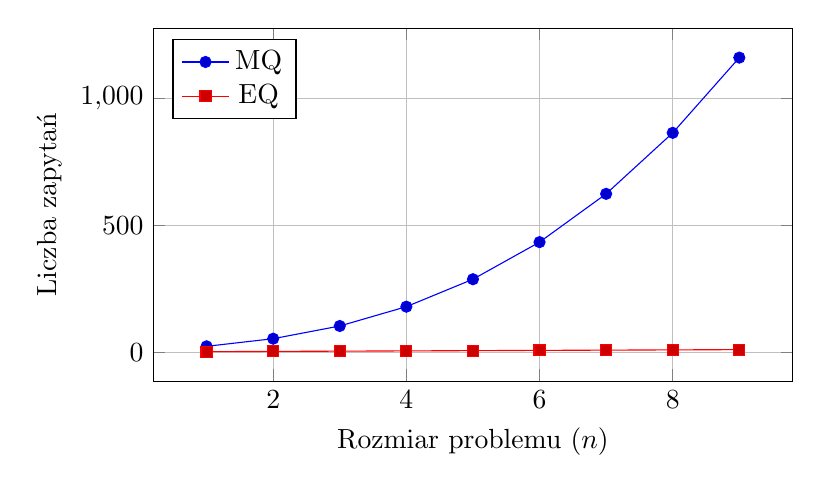
\begin{tikzpicture}
\begin{axis}[
    xlabel={Rozmiar problemu (\(n\))},
    ylabel={Liczba zapytań},
    legend pos=north west,
    grid=major,
    width=0.8\textwidth,
    height=0.5\textwidth
]

% MQ
\addplot coordinates {(1, 24) (2, 54) (3, 104) (4, 180) (5, 288) (6, 434) (7, 624) (8, 864) (9, 1160)};
\addlegendentry{MQ}

% EQ
\addplot coordinates {(1, 3) (2, 4) (3, 5) (4, 6) (5, 7) (6, 8) (7, 9) (8, 10) (9, 11)};
\addlegendentry{EQ}

\end{axis}
\end{tikzpicture}
\caption{Zależność liczby zapytań EQ i MQ od rozmiaru problemu dla języka z sekcji \ref{sec:eksperyment2}.}
\label{fig:lstar_blocks_mq}
\end{figure}


\section{Algorytm \textit{RPNI}}  
Eksperymenty dla algorytmu \textit{RPNI} miały na celu ocenę wpływu rozmiaru alfabetu na czas działania oraz strukturę wynikowego automatu. Testy przeprowadzono na językach z ciągami rozpoczynającymi się symbolem \( 0 \), po którym mogły występować dowolne symbole z danego alfabetu. Dane testowe przygotowano tak, aby liczba stanów w drzewie prefiksów (\textit{PTA}) była zbliżona dla różnych konfiguracji, co zapewniło porównywalność wyników.  

Tabela \ref{tab:rpni_results} przedstawia szczegóły wyników eksperymentu. Kolumna \textit{Rozmiar alfabetu (\(|\Sigma|\))} określa liczbę symboli w alfabecie testowego języka, a \textit{Liczba przykładów} podaje łączną liczbę danych wejściowych. Kolumny \textit{Stany PTA} i \textit{Stany DFA} przedstawiają odpowiednio liczbę stanów w drzewie prefiksów i wynikowym automacie deterministycznym (\textit{DFA}). Ostatnia kolumna, \textit{Czas [s]}, zawiera czas wykonania algorytmu.  

Wyniki pokazują, że czas działania algorytmu rośnie wraz z rozmiarem alfabetu (rys. \ref{fig:rpni_time}), choć dla alfabetu o rozmiarze 64 odnotowano krótszy czas niż dla 32. Może to wynikać ze specyfiki danych testowych lub procesu łączenia stanów. Liczba stanów w wynikowym automacie pozostaje niska, co świadczy o skuteczności algorytmu w uogólnianiu danych, jednak dla większych alfabetów (\(|\Sigma| = 16\) i \(|\Sigma| = 32\)) obserwuje się niewielki wzrost liczby stanów, co może sugerować trudności w uogólnianiu przypadków ze średnim rozmiarem alfabetu.  

Porównywalna liczba stanów w \textit{PTA} dla różnych rozmiarów alfabetów zapewniła rzetelność wyników, eliminując wpływ różnic w danych wejściowych. Algorytm \textit{RPNI} zachowuje wydajność przy różnych konfiguracjach parametrów, choć czas działania rośnie dla większych alfabetów.

\begin{table}[h]
\centering
\caption{Wyniki dla algorytmu \textit{RPNI}.}
\label{tab:rpni_results}
\begin{tabular}{|c|c|c|c|c|}
\hline
Rozmiar alfabetu (\(|\Sigma|\)) & Liczba przykładów & Stany PTA & Stany DFA & Czas [s] \\ \hline
2                               & 2807              & 5508.44   & 3         & 0.104656 \\ \hline
4                               & 1821              & 4993.48   & 3         & 0.166168 \\ \hline
8                               & 1673              & 5675.68   & 3         & 0.364098 \\ \hline
16                              & 1673              & 5307.78   & 3.58      & 0.644382 \\ \hline
32                              & 2257              & 5103.64   & 4.50      & 1.080040 \\ \hline
64                              & 4561              & 4756.92   & 3.06      & 0.883063 \\ \hline
\end{tabular}
\end{table}

\begin{figure}[h]
\centering
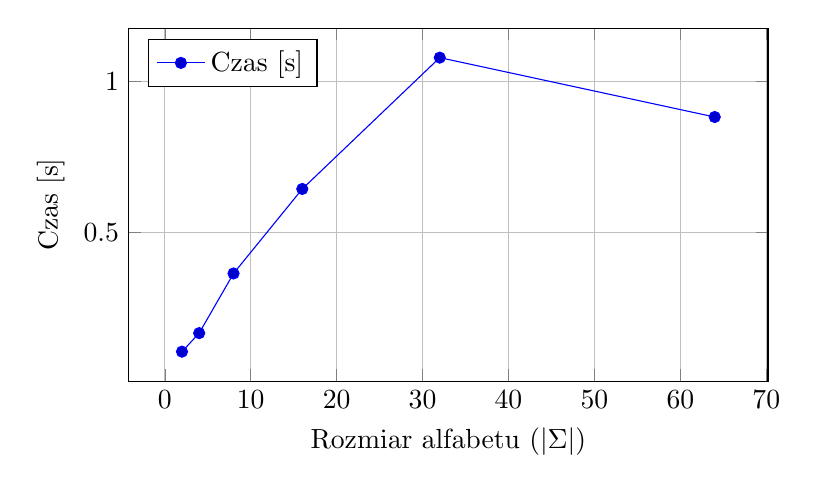
\begin{tikzpicture}
\begin{axis}[
    xlabel={Rozmiar alfabetu (\(|\Sigma|\))},
    ylabel={Czas [s]},
    legend pos=north west,
    grid=major,
    width=0.8\textwidth,
    height=0.5\textwidth
]
\addplot coordinates {(2, 0.104656) (4, 0.166168) (8, 0.364098) (16, 0.644382) (32, 1.08004) (64, 0.883063)};
\addlegendentry{Czas [s]}
\end{axis}
\end{tikzpicture}
\caption{Zależność czasu wykonania algorytmu RPNI od rozmiaru alfabetu.}
\label{fig:rpni_time}
\end{figure}


\section{Algorytm \textit{GIG}}  
Przeprowadzone eksperymenty dla algorytmu \textit{GIG} miały na celu zbadanie wpływu metody inicjalizacji populacji na jakość wynikowego automatu, liczbę generacji potrzebnych do uzyskania rozwiązania oraz dokładność klasyfikacji danych testowych.

Tabele \ref{tab:gig_one_a}, \ref{tab:gig_even_a} oraz \ref{tab:gig_even_a_or_b} prezentują wyniki uzyskane dla różnych metod inicjalizacji populacji. Kolumna \textit{Inicjalizacja populacji} określa zastosowany sposób inicjalizacji – \textit{warstwowa} oznacza podejście opisane w sekcji \ref{sec:gig-formalizacja}, natomiast \textit{losowa} generuje populację bez dodatkowych założeń. Kolumna \textit{Pokolenie} przedstawia średnią liczbę pokoleń potrzebnych do znalezienia rozwiązania. Kolumna \textit{Jakość} podaje skuteczność modelu jako procent poprawnych klasyfikacji. Kolumny \textit{TP} (True Positives) i \textit{TN} (True Negatives) wskazują odsetek poprawnych klasyfikacji przykładów pozytywnych i negatywnych, natomiast kolumny \textit{FP} (False Positives) i \textit{FN} (False Negatives) pokazują odsetek błędnych klasyfikacji.

Obie metody inicjalizacji populacji osiągnęły wysoką jakość klasyfikacji w każdym teście, lecz metoda losowa przyniosła lepsze rezultaty, skracając czas konwergencji średnio o $5.42$ pokolenia w teście trzecim (tabela \ref{tab:gig_even_a_or_b}). Sugeruje to, że losowość skuteczniej eksploruje przestrzeń rozwiązań, zwiększając prawdopodobieństwo znalezienia optymalnych modeli. 

Analiza wyników pokazuje, że metoda losowej inicjalizacji była bardziej efektywna dla złożonych języków, podczas gdy dla prostszych obie metody osiągały podobne rezultaty. Różnice w liczbie generacji okazały się niewielkie, co wskazuje, że wybór metody inicjalizacji miał większy wpływ na jakość wynikowych modeli niż na tempo konwergencji algorytmu.


\begin{table}[h]
\centering
\caption{Wyniki dla języka „Co najmniej jedno \( a \)” z sekcji \ref{sec:eksperyment4}.}
\label{tab:gig_one_a}
\begin{tabular}{|l|c|c|c|c|c|c|}
\hline
Inicjalizacja populacji & Pokolenie & Jakość & TP & TN & FP & FN \\ \hline
Inicjalizacja warstwowa & 94.64 & 0.944 & 0.889 & 1 & 0.111 & 0 \\ \hline
Inicjalizacja losowa    & 91.46 & 0.943 & 0.887 & 1 & 0.113 & 0 \\ \hline
\end{tabular}
\end{table}

\begin{table}[h]
\centering
\caption{Wyniki dla języka „Parzysta liczba \( a \)” z sekcji \ref{sec:eksperyment5}.}
\label{tab:gig_even_a}
\begin{tabular}{|l|c|c|c|c|c|c|}
\hline
Inicjalizacja populacji & Pokolenie & Jakość & TP & TN & FP & FN \\ \hline
Inicjalizacja warstwowa & 95.7  & 0.974 & 1 & 0.945 & 0 & 0.055 \\ \hline
Inicjalizacja losowa    & 96.44 & 0.987 & 1 & 0.973 & 0 & 0.028 \\ \hline
\end{tabular}
\end{table}

\begin{table}[h]
\centering
\caption{Wyniki dla języka „Parzysta liczba \( a \) lub \( b \)” z sekcji \ref{sec:eksperyment6}.}
\label{tab:gig_even_a_or_b}
\begin{tabular}{|l|c|c|c|c|c|c|}
\hline
Inicjalizacja populacji & Pokolenie & Jakość & TP & TN & FP & FN \\ \hline
Inicjalizacja warstwowa & 96.2  & 0.923 & 0.97  & 0.875 & 0.03  & 0.125 \\ \hline
Inicjalizacja losowa    & 90.78 & 0.968 & 0.988 & 0.948 & 0.013 & 0.053 \\ \hline
\end{tabular}
\end{table}


\section{Algorytm \textit{ALERGIA}}  
Badania nad algorytmem \textit{ALERGIA} skupiały się na ocenie jego odporności na szum w danych wejściowych. Analizowano jakość wynikowego modelu oraz liczbę stanów w wynikowym automacie w zależności od poziomu zakłóceń.

Podsumowanie wyników eksperymentu przedstawiono w tabeli \ref{tab:alergia_results}. Kolumna \textit{Procent szumu} określa poziom zakłóceń w danych wejściowych. Kolumna \textit{Jakość} podaje dokładność modelu jako odsetek poprawnych klasyfikacji wśród 10000 słów wygenerowanych z wynikowego automatu. Kolumna \textit{Stany automatu} wskazuje liczbę stanów w wynikowym automacie, co pozwala ocenić złożoność struktury modelu. Wszystkie wartości są uśrednione na podstawie powtórzeń testu.

Jak pokazują tabela \ref{tab:alergia_results} oraz wykresy \ref{fig:alergia_quality} i \ref{fig:alergia_states}, jakość modelu spada wraz ze wzrostem poziomu szumu w danych. Dla niskich zakłóceń (do 2\%) algorytm utrzymuje jakość powyżej 89\%, jednak przy 50\% szumu dokładność spada do około 74\%.  

Liczba stanów w wynikowym automacie wzrasta wraz z poziomem zakłóceń, co wskazuje na trudności w uogólnianiu danych przy większym szumie. Przy zakłóceniach do 10\% liczba stanów pozostaje stabilna, natomiast przy wyższych wartościach rośnie zauważalnie, odzwierciedlając większą złożoność modelu.

Wyniki eksperymentów pokazują, że algorytm \textit{ALERGIA} dobrze radzi sobie z niewielkimi zakłóceniami, zachowując wysoką jakość klasyfikacji i kompaktową strukturę automatu. W miarę wzrostu poziomu szumu jego zdolność do poprawnego odwzorowania języka stopniowo maleje, co objawia się zarówno spadkiem dokładności, jak i wzrostem liczby stanów automatu.

\begin{table}[h]
\centering
\caption{Wyniki dla algorytmu \textit{ALERGIA}.}
\label{tab:alergia_results}
\begin{tabular}{|c|c|c|}
\hline
Procent szumu & Jakość & Stany automatu \\ \hline
0             & 1.0000 & 2             \\ \hline
0.001         & 0.9941 & 2             \\ \hline
0.005         & 0.9734 & 2.14          \\ \hline
0.01          & 0.9527 & 2.56          \\ \hline
0.02          & 0.9280 & 3.30           \\ \hline
0.05          & 0.8921 & 3.92          \\ \hline
0.1           & 0.8985 & 4             \\ \hline
0.2           & 0.9100 & 4             \\ \hline
0.3           & 0.8664 & 4.32          \\ \hline
0.4           & 0.7998 & 4.98          \\ \hline
0.5           & 0.7412 & 5.36          \\ \hline
\end{tabular}
\end{table}

\begin{figure}[h]
\centering
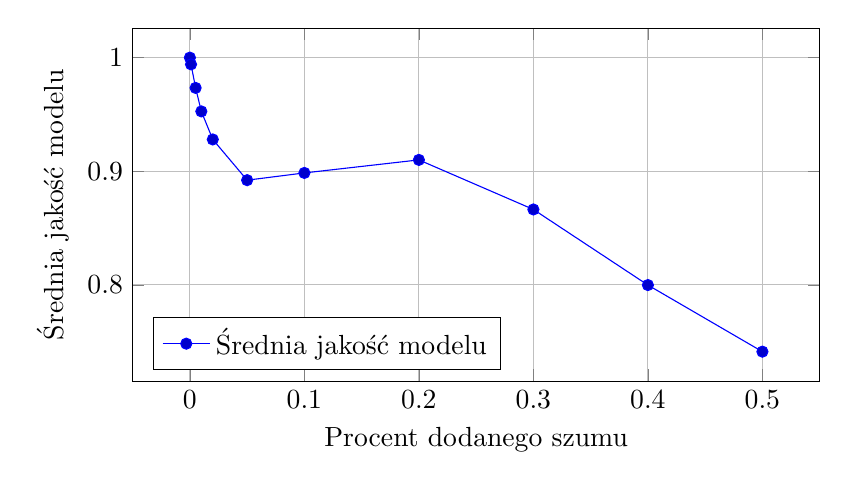
\begin{tikzpicture}
\begin{axis}[
    xlabel={Procent dodanego szumu},
    ylabel={Średnia jakość modelu},
    legend pos=south west,
    grid=major,
    width=0.85\textwidth,
    height=0.5\textwidth
]
\addplot coordinates {(0, 1.0) (0.001, 0.994074) (0.005, 0.97336) (0.01, 0.95268) (0.02, 0.927988) (0.05, 0.892144) (0.1, 0.898522) (0.2, 0.909984) (0.3, 0.866366) (0.4, 0.799828) (0.5, 0.741206)};
\addlegendentry{Średnia jakość modelu}
\end{axis}
\end{tikzpicture}
\caption{Zależność jakości modelu od poziomu szumu w danych.}
\label{fig:alergia_quality}
\end{figure}

\begin{figure}[h]
\centering
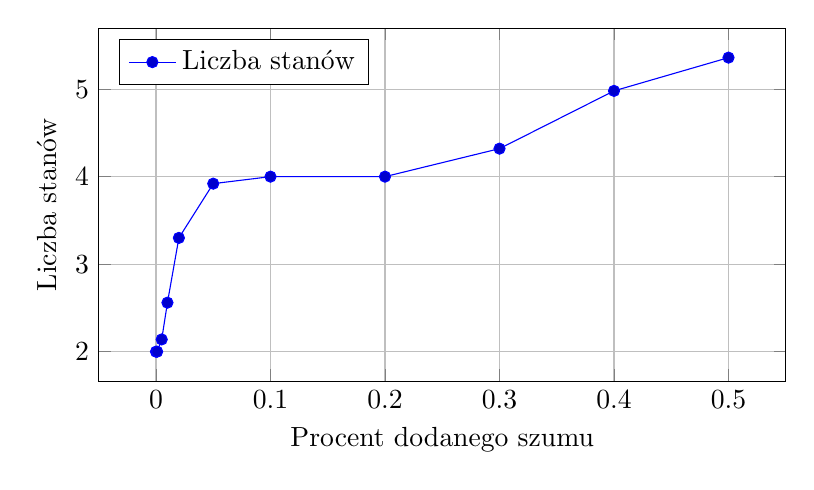
\begin{tikzpicture}
\begin{axis}[
    xlabel={Procent dodanego szumu},
    ylabel={Liczba stanów},
    legend pos=north west,
    grid=major,
    width=0.85\textwidth,
    height=0.5\textwidth
]
\addplot coordinates {(0, 2) (0.001, 2) (0.005, 2.14) (0.01, 2.56) (0.02, 3.3) (0.05, 3.92) (0.1, 4) (0.2, 4) (0.3, 4.32) (0.4, 4.98) (0.5, 5.36)};
\addlegendentry{Liczba stanów}
\end{axis}
\end{tikzpicture}
\caption{Zależność liczby stanów wynikowego automatu od poziomu szumu dodanego do danych.}
\label{fig:alergia_states}
\end{figure}


\section{Podsumowanie}  
Przeprowadzone eksperymenty pozwoliły na ocenę skuteczności i wydajności algorytmów \textit{L*}, \textit{RPNI}, \textit{GIG} oraz \textit{ALERGIA}. Algorytm \textit{L*} efektywnie generował minimalne automaty deterministyczne (\textit{DFA}), utrzymując niską liczbę zapytań o równoważność (\textit{EQ}), choć liczba zapytań o przynależność (\textit{MQ}) rosła wykładniczo wraz ze złożonością problemu, co czyni go odpowiednim w sytuacjach z dobrze zdefiniowanymi źródłami wiedzy. Algorytm \textit{RPNI} wyróżniał się prostotą, niską złożonością i wysoką wydajnością, co czyni go dobrym wyborem do szybkiego uogólniania danych, niezależnie od rozmiaru alfabetu. Algorytm \textit{GIG}, oparty na metodach ewolucyjnych, oferował elastyczność, lecz jego większa złożoność i czasochłonność nie zawsze przekładały się na lepsze wyniki w porównaniu z prostszymi metodami, a eksperymenty wykazały, że losowa inicjalizacja populacji częściej prowadziła do lepszych wyników niż inicjalizacja warstwowa. Algorytm \textit{ALERGIA} okazał się odporny na niewielkie zakłócenia, zachowując wysoką jakość klasyfikacji i kompaktową strukturę modelu, jednak jego skuteczność spadała przy większym poziomie szumu, co czyni go bardziej odpowiednim do danych probabilistycznych o umiarkowanym poziomie zakłóceń. Wybór algorytmu powinien być zatem dostosowany do specyfiki problemu – \textit{L*} sprawdza się tam, gdzie dostępna jest wyrocznia wysokiej jakości, \textit{RPNI} oferuje szybkość i prostotę, \textit{GIG} nadaje się do złożonych problemów optymalizacyjnych, a \textit{ALERGIA} jest przydatna w modelowaniu danych probabilistycznych.

    \chapter{Podsumowanie}
\label{cha:podsumowanie}  

Praca poświęcona była analizie zachowania i porównaniu czterech algorytmów indukcji gramatyk formalnych: \textit{RPNI}, \textit{L*}, \textit{ALERGIA} oraz \textit{GIG}. W jej ramach stworzono środowisko eksperymentalne, które umożliwiło ocenę tych metod pod kątem wydajności, dokładności oraz zdolności do uogólniania danych. Implementacja została zrealizowana w języku Python z wykorzystaniem bibliotek \textit{aalpy}, \textit{pygad}, \textit{numpy}, \textit{automata-lib} oraz \textit{pydot}, co pozwoliło na przeprowadzenie eksperymentów i wizualizację wyników.

Wykonana praca obejmuje opracowanie implementacji algorytmu \textit{GIG} z wykorzystaniem frameworku \textit{pygad}. W ramach tej implementacji autor zaadaptował operacje genetyczne, takie jak krzyżowanie i mutacja, opracował funkcje generujące populacje oraz zdefiniował funkcję przystosowania (\textit{fitness function}). Ponadto, zaimplementowano moduły uruchamiające eksperymenty, odpowiedzialne za konfigurację parametrów testowych i inicjalizację ich przebiegu. Oprócz tego autor stworzył funkcje wspomagające, takie jak mechanizmy generowania zbiorów danych, dodawania szumu do danych oraz obliczania jakości modeli. Kod został zaprojektowany w sposób umożliwiający jego rozszerzanie oraz ponowne wykorzystanie w przyszłych badaniach.  

Eksperymenty pozwoliły na ocenę skuteczności i wydajności badanych algorytmów. Algorytm \textit{L*} generował minimalne automaty deterministyczne (\textit{DFA}) przy niskiej liczbie zapytań o równoważność (\textit{EQ}), jednak liczba zapytań o przynależność (\textit{MQ}) rosła wykładniczo wraz ze złożonością problemu. Algorytm \textit{RPNI} wyróżniał się prostotą, niską złożonością i skutecznym uogólnianiem danych. Algorytm \textit{GIG}, choć oferował elastyczność dzięki zastosowaniu metod ewolucyjnych, nie zawsze przewyższał prostsze metody pod względem wyników, a losowa inicjalizacja populacji często prowadziła do lepszych rezultatów niż inicjalizacja warstwowa. Algorytm \textit{ALERGIA} wykazał odporność na niewielkie zakłócenia, jednak jego skuteczność malała wraz ze wzrostem poziomu szumu, co czyni go bardziej odpowiednim dla danych probabilistycznych o umiarkowanym poziomie zakłóceń.  

W trakcie realizacji pracy napotkano kilka wyzwań teoretycznych i praktycznych, które wymagały odpowiednich rozwiązań. Pierwszym problemem była ocena jakości modeli stochastycznych. Standardowe metryki, takie jak macierz pomyłek, nie mogły zostać zastosowane z uwagi na probabilistyczny charakter automatu. Rozwiązaniem było generowanie dużej liczby losowych zdań z automatu wynikowego i ich weryfikacja przez poprawny automat referencyjny. Pozwoliło to na przybliżoną ocenę jakości modeli.

Kolejnym wyzwaniem była sprawiedliwa ocena czasu działania algorytmu \textit{RPNI} w zależności od rozmiaru alfabetu. Czas działania algorytmu zależy od liczby stanów w akceptorze prefiksów (\textit{PTA}), która z kolei wynika z liczby i długości przykładów w danych wejściowych. Liczba stanów w \textit{PTA} jest trudna do przewidzenia i różni się w zależności od alfabetu, co utrudniało porównanie wyników. Problem rozwiązano poprzez ręczne dobieranie liczby przykładów, tak aby liczba stanów w \textit{PTA} była porównywalna dla różnych rozmiarów alfabetów.

Największym wyzwaniem w przypadku algorytmu \textit{GIG} było dobranie odpowiedniej funkcji przystosowania (\textit{fitness function}). Zbyt duży nacisk na minimalizację liczby stanów w automacie prowadził do utraty dokładności klasyfikacji, podczas gdy priorytetowanie poprawności klasyfikacji skutkowało generowaniem nadmiernie złożonych modeli. Rozwiązaniem okazało się empiryczne dostosowanie funkcji przystosowania, które uwzględniało zarówno minimalizację automatu, jak i jego dokładność. Funkcja wymagała jednak dopasowywania do specyfiki każdego przypadku, co wskazuje na potrzebę dalszych badań w tym obszarze.

Podsumowując, praca pozwoliła na stworzenie wszechstronnego środowiska testowego oraz przeprowadzenie szczegółowej analizy porównawczej algorytmów indukcji gramatyk formalnych. Wyniki eksperymentów wskazują na konieczność dopasowania wyboru algorytmu do specyfiki problemu i charakterystyki danych. Środowisko jest gotowe do dalszej rozbudowy, a przyszłe badania mogą objąć testy na danych rzeczywistych, optymalizację obecnych metod oraz analizę dodatkowych algorytmów.


\section{Dalsze kierunki rozwoju}
Możliwości dalszego rozwoju obejmują powtórzenie eksperymentów na bardziej złożonych lub rzeczywistych danych, co pozwoliłoby na dokładniejsze zbadanie praktycznych zastosowań algorytmów. Ponadto warto przeprowadzić dodatkowe analizy dla innych metod indukcji gramatyk formalnych, które nie zostały uwzględnione w tej pracy, w celu poszerzenia porównania i oceny ich skuteczności w różnych warunkach.

    
    % \appendix
    % \include{dodatek}
    % itd.
    
    \printbibliography

\end{document}
